\documentclass[5pt,aspectratio=169]{beamer}
\usetheme{metropolis}
\metroset{block=fill}
%\usecolortheme{whale}
\usepackage{tikz}
\usetikzlibrary{decorations.pathmorphing}
\usepackage{listings}
\usepackage{amsmath}
\usepackage{xcolor}
\usepackage[normalem]{ulem} % Provides \sout for strikeout
\usepackage{attachfile}
\usetikzlibrary{arrows,shapes,positioning,fit,arrows.meta,backgrounds,calc}

% Code listing setup
\lstset{
  basicstyle=\footnotesize\ttfamily,
  breaklines=true,
  commentstyle=\color{green!60!black},
  keywordstyle=\color{blue},
  stringstyle=\color{red},
  numbers=left,
  numberstyle=\tiny\color{gray},
  backgroundcolor=\color{gray!10},
  frame=single,
  tabsize=2
}

\title{Foundations of Deep Learning \& the Emergence of Generative AI}
%\subtitle{Session 1}
\author{Mari Ganesh Kumar}
\date{\today}
%\institute{[Institution]}

\begin{document}

%% Title Slide
\begin{frame}
\titlepage
\end{frame}

%% Slide 3: Learning Objectives



\begin{frame}
\frametitle{Course Outline}
\begin{itemize}
    \item Foundations of Deep Learning \& Emergence of Generative AI
    \item VAEs
    \item GANs
    \item Auto-regressive generative models
\end{itemize}
\end{frame}

\section{Course Overview \& State of the Art}

\begin{frame}
    \begin{figure}
        \centering
        
\includegraphics[width=0.5\linewidth]{images/image.png}
        \label{fig:enter-label}
    \end{figure}
    \centering
     \href{https://forms.gle/C5ka9tqLZQnzY9Qx7}{click here}
\end{frame}


\begin{frame}
\frametitle{Session Learning Objectives}
By the end of this session, you will be able to:
\begin{itemize}
    \item Understand the evolution from traditional ML to deep learning
    \item Explain fundamental neural network architectures and their components
    \item Describe how deep learning innovations led to generative AI
    \item Implement a basic autoencoder for image reconstruction
\end{itemize}
\end{frame}

\begin{frame}
\frametitle{%
    \alt<1>{What is Generative AI?}{%
      \alt<2>{What is Generative \texorpdfstring{\sout{AI} Modeling}{AI}?}{%
        \texorpdfstring{What is a simple Generative \sout{AI Modeling} Model?}{Generative Modeling}}%
    }%
  }

\begin{itemize}
\item<4-> Observed Data
\[
X: H, T, H, H, T
\]
\item<5-> How can we continue generating data based on observed data?
\[
\hat{X}: H, T, H, H, T, ?, ?, ?, ?
\]
\item<6-> Let's compress the data into a parameter (not using ML simple Math)
\[
\theta = \frac{\#\text{Heads}}{N} = \frac{3}{5} = 0.6
\]
\item<7-> Let's compress the data into a parameter (in ML world)
\[
\text{maximize likelihood of $\theta $  } \rightarrow \; \arg\max_{\theta}L(\theta; X) = \arg\max_{\theta}\prod_{i=1}^{n} \theta^{x_i}(1-\theta)^{1-x_i} = 0.6
\]
\end{itemize}
\end{frame}

\begin{frame}
\frametitle{%
        \texorpdfstring{What is a simple Generative \sout{AI Modeling} Model?}{Generative Modeling}%
  }

\begin{itemize}
\item<1-> Observed Data
\[
X: H, T, H, H, T
\]
\item<1-> How can we continue generating data based on observed data?
\[
\hat{X}: H, T, H, H, T, ?, ?, ?, ?
\]
\item<1-> We compressed the data into a parameter (  $\theta = 0.6 $)
\item<2-> How do we generate data using $\theta$ 
\begin{itemize}
\item<3->$\text{Generate } u \text{ as a random number between } 0  \text{ and } 1 \text{. If } u<\theta \text{, then }\hat{X}=H\text{; else, }\hat{X}=T$
\end{itemize}
\end{itemize}
\end{frame}

% \begin{frame}{What is Generative Modelling?}
% \begin{itemize}
%     \item H,T,T,H,H,.. ->[]-> $\theta$ ->[] ->   Generated data
%     \item Image-1, Image-2, Image-3 ->[Model Training]-> $\theta$ -> [Inference] ->   Generated data
%     \item Text, Text, Text ->[Model Training]-> $\theta$ -> [Inference] ->   Generated data
    
% \end{itemize}
    
% \end{frame}



\begin{frame}{What is Generative Modelling?}
\begin{itemize}
    \item \textbf{Coin Flips}
    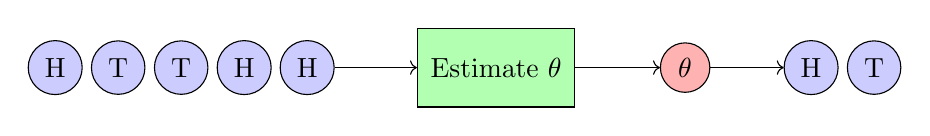
\begin{tikzpicture}[scale=0.8]
        % Original data
        \node[draw,circle,fill=blue!20] (h1) at (0,0) {H};
        \node[draw,circle,fill=blue!20] (t1) at (1,0) {T};
        \node[draw,circle,fill=blue!20] (t2) at (2,0) {T};
        \node[draw,circle,fill=blue!20] (h2) at (3,0) {H};
        \node[draw,circle,fill=blue!20] (h3) at (4,0) {H};
        
        % Model training
        \node[draw,rectangle,fill=green!30,minimum width=2cm,minimum height=1cm] (model) at (7,0) {Estimate $\theta$};
        \node[draw,circle,fill=red!30] (theta) at (10, 0) {$\theta$};
        
        % Generated data
        \node[draw,circle,fill=blue!20] (gh1) at (12,0) {H};
        \node[draw,circle,fill=blue!20] (gt1) at (13,0) {T};
        
        % Arrows
        \draw[->] (h3) -- (model);
        \draw[->] (model) -- (theta);
        \draw[->] (theta) -- (gh1);
        %\draw[->] (theta) -- (gt1);
    \end{tikzpicture}
    
    \item \textbf{Image Generation Example:}
    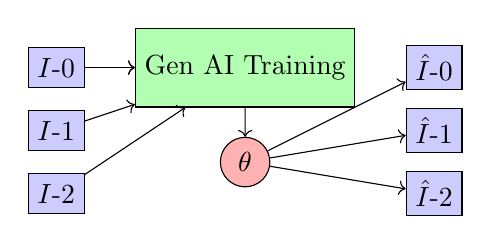
\begin{tikzpicture}[scale=0.8]
        % Original images
        \foreach \i in {0,1,2} {
            \node[draw,rectangle,fill=blue!20,minimum size=0.5cm] (I\i) at (0,-\i) {$I$-\i};
        }
        
        % Model training
        \node[draw,rectangle,fill=green!30,minimum width=2cm,minimum height=1cm] (model) at (3,0) {Gen AI Training};
        \node[draw,circle,fill=red!30] (theta) at (3,-1.5) {$\theta$};
        
        % Generated image
        \foreach \i in {0,1,2} {
            \node[draw,rectangle,fill=blue!20,minimum size=0.5cm] (i\i) at (6,-\i) {$\hat{I}$-\i};
        }

        
        % Arrows
        \foreach \i in {0,1,2} {
            \draw[->] (I\i) -- (model);
            \draw[->] (theta) -- (i\i);
        }
        \draw[->] (I0) -- (model);
        \draw[->] (model) -- (theta);
    \end{tikzpicture}
    
    \item \textbf{Text Generation Example:}
    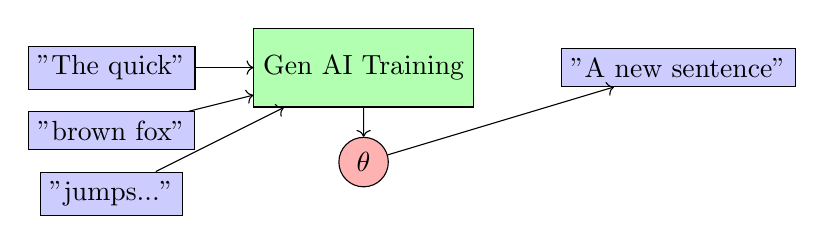
\begin{tikzpicture}[scale=0.8]
        % Original text
        \node[draw,rectangle,fill=blue!20] (text1) at (0,0) {"The quick"};
        \node[draw,rectangle,fill=blue!20] (text2) at (0,-1) {"brown fox"};
        \node[draw,rectangle,fill=blue!20] (text3) at (0,-2) {"jumps..."};
        
        % Model training
        \node[draw,rectangle,fill=green!30,minimum width=2cm,minimum height=1cm] (model) at (4,0) {Gen AI Training};
        \node[draw,circle,fill=red!30] (theta) at (4,-1.5) {$\theta$};
        
        % Generated text
        \node[draw,rectangle,fill=blue!20] (gtext) at (9,0) {"A new sentence"};
        
        % Arrows
         \foreach \i in {1,2,3} {
            \draw[->] (text\i) -- (model);
        }
        \draw[->] (model) -- (theta);
        \draw[->] (theta) -- (gtext);
    \end{tikzpicture}
\end{itemize}
\end{frame}

\begin{frame}{What is Generative AI?}

\begin{center}
\large{Common Pattern: Data $\rightarrow$ Learn Parameters $\rightarrow$ Generate New Samples}
\end{center}
\only<2->{
Today's GEN AI models can learn and generate any data (to a decent accuracy)
\begin{itemize}
    \item<3-> Generate Code, Code which solves a given task, Generate testcases given code 
    \item<4-> Generate Images, Videos, Speech, Music and turn any given image into a Ghlibli style
    \item<5-> Generate movements for a robot to navigate the physical world
    \item etc,etc
\end{itemize}
}
\only<3->{These models are getting better that all the above tasks, as we speak}
    
\end{frame}


\begin{frame}{Generative AI: The State of the Art (2024–2026)}
\begin{columns}[T]
\begin{column}{0.48\textwidth}
    \begin{block}{1. Reasoning \& Logic (GPT-4o)}
        \footnotesize
        \textbf{Prompt:} "If a shirt takes 1 hour to dry in the sun, how long for 50 shirts?" \\
        \textbf{Output:} "1 hour, as they can all be dried at once." 
    \end{block}
    \vspace{0.2cm}
    \begin{block}{3. Audio (Suno / Udio)}
        \footnotesize
        \textbf{Prompt:} "Generate a Gen AI anthem in \textbf{Anirudh Style} (High-energy rock/EDM)." \\
        \textit{[Generates full instrumentation and vocals]}
    \end{block}
\end{column}
\begin{column}{0.48\textwidth}
    \begin{block}{2. Image (Midjourney / DALL-E 3)}
        \centering
        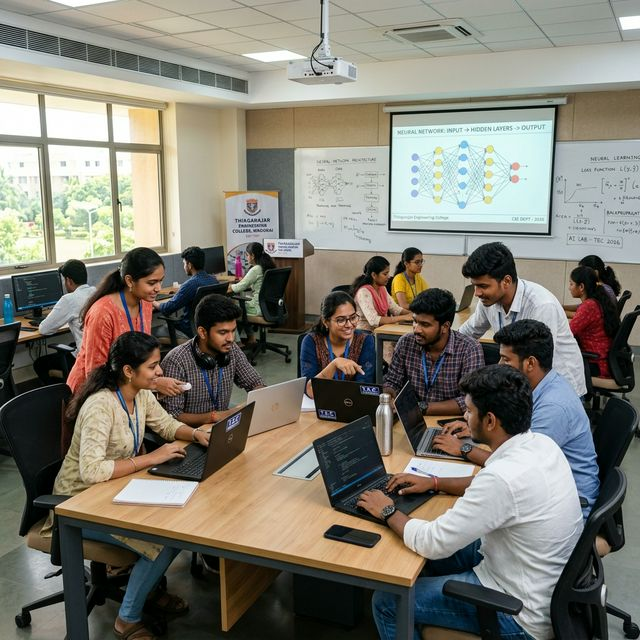
\includegraphics[width=0.9\linewidth]{images/tce_classroom_2026.png} \\
        \tiny \textit{"TCE Madurai Classroom, 2026"}
    \end{block}
    \vspace{0.1cm}
    \begin{block}{4. Video (Sora / Kling / Luma / Kling)}
        \footnotesize
        \textbf{Prompt:} "Cinematic slow-motion video explaining the coin toss in the context of Gen AI." \\
        \textit{[Physics-aware video generation]}
    \end{block}
\end{column}
\end{columns}
\end{frame}



\section{The Birth of Neural Networks}
\subsection{From ML to Deep Learning}
%% Slide 6: Traditional ML vs Deep Learning
\begin{frame}
\frametitle{From Traditional ML to Deep Learning}
\begin{columns}
\begin{column}{0.48\textwidth}
\textbf{Traditional Machine Learning:}
\begin{itemize}
    \item Relies on hand-crafted features
    \item Limited ability to process raw data
    \item Requires extensive feature engineering
    \item Often plateaus with more data
\end{itemize}
\end{column}
\begin{column}{0.48\textwidth}
\textbf{Deep Learning:}
\begin{itemize}
    \item Automatic feature extraction
    \item Works directly with raw data
    \item Features learned hierarchically
    \item Scales with data and compute
\end{itemize}
\end{column}
\end{columns}
\end{frame}

\subsection{The Perceptron (1940s-1950s)}

%% Slide 7: History of Deep Learning
\begin{frame}
\frametitle{Brief History of Deep Learning}
\begin{itemize}
    \item 1940s-50s: McCulloch, Pitts, and Rosenblatt develop perceptron
    \item 1980s: Backpropagation algorithm formalized
    \item 1990s: LeCun develops LeNet for digit recognition
    \item 2006: Hinton introduces deep belief networks
    \item 2012: AlexNet wins ImageNet competition
    \item 2014-present: Explosion of deep learning research and applications
\end{itemize}
\end{frame}

%%% 1940s-1950s: Perceptron Foundations %%%
\begin{frame}
\frametitle{1940s-1950s: Birth of Artificial Neurons}

\begin{columns}[T]
\begin{column}{0.5\textwidth}
\textbf{Key Developments:}
\begin{itemize}
\item \textbf{1943:} McCulloch-Pitts Neuron
\begin{itemize}
\item First mathematical model of biological neurons
\item Binary threshold function: 
\( f(x) = \begin{cases} 
1 & \text{if } \sum w_i x_i \geq \theta \\
0 & \text{otherwise}
\end{cases} \)
\end{itemize}

\item \textbf{1958:} Rosenblatt's Perceptron
\begin{itemize}
\item First learning algorithm for neural networks
\item \textbf{Limitations:}
\begin{itemize}
\item Could only learn linearly separable patterns
\end{itemize} 

\end{itemize}
\end{itemize}
\end{column}

\begin{column}{0.5\textwidth}
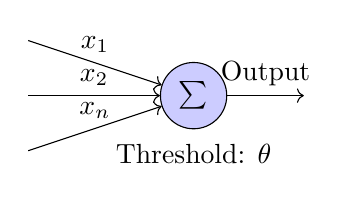
\begin{tikzpicture}[scale=0.7]
\node[draw,circle,fill=blue!20] (neuron) at (1,0) {$\sum$};
\draw[->] (-2,1) -- (neuron) node[midway,above] {$x_1$};
\draw[->] (-2,0) -- (neuron) node[midway,above] {$x_2$};
\draw[->] (-2,-1) -- (neuron) node[midway,above] {$x_n$};
\draw[->] (neuron) -- (3,0) node[midway,above] {Output};
\node[below=0.5cm] at (neuron) {Threshold: $\theta$};
\end{tikzpicture}

\vspace{0.5cm}
\textbf{Learning Rule:}
\begin{itemize}
    \item 
  \[
  w_i \leftarrow w_i + \eta(y - \hat{y})x_i
  \]
  \small{where \(\eta\) = learning rate, \(y\) = target, \(\hat{y}\) = prediction}
\item Iterative weight updates until convergence
\item Guaranteed to converge for linearly separable data
\end{itemize}

\end{column}
\end{columns}
\end{frame}



%%% Slide 1: Linear Classification Example %%%
\begin{frame}
\frametitle{Perceptron: Linear Classification Example}

\begin{columns}[T]
\begin{column}{0.5\textwidth}
\textbf{AND Gate Problem:}
\begin{itemize}
\item Inputs: \(x_1, x_2 \in \{0,1\}\)
\item Target: \(y = x_1 \land x_2\)
\end{itemize}

\textbf{Learning Process:}
\begin{enumerate}
\item Initialize weights: \(w_1=0.2, w_2=0.5, \theta=0.7\)
\item For each training example:
\begin{itemize}
\item Compute output: 
\(\hat{y} = \begin{cases} 
1 & \text{if } w_1x_1 + w_2x_2 \geq \theta \\
0 & \text{otherwise}
\end{cases}\)
\item Update weights: 
\(\Delta w_i = \eta(y - \hat{y})x_i\)
\end{itemize}
\end{enumerate}
\end{column}

\begin{column}{0.5\textwidth}
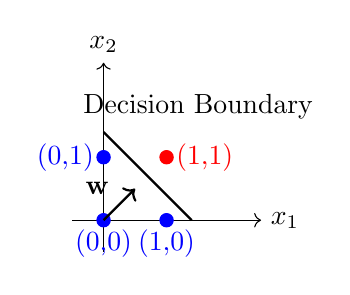
\begin{tikzpicture}[scale=0.8]
% Decision boundary: 0.5x + 0.5y = 0.7 => y = 1.4 - x
\draw[->] (-0.5,0) -- (2.5,0) node[right] {$x_1$};
\draw[->] (0,-0.5) -- (0,2.5) node[above] {$x_2$};
\draw[thick] (0.7/0.5,0) -- (0,0.7/0.5);
\node at (1.5,1.8) {Decision Boundary};

% AND gate points
\filldraw[blue] (0,0) circle (3pt) node[below] {(0,0)};
\filldraw[blue] (0,1) circle (3pt) node[left] {(0,1)};
\filldraw[blue] (1,0) circle (3pt) node[below] {(1,0)};
\filldraw[red] (1,1) circle (3pt) node[right] {(1,1)};

% Weight vector
\draw[->,thick] (0,0) -- (0.5,0.5) node[midway,above left] {\(\mathbf{w}\)};
\end{tikzpicture}

\begin{itemize}
\item Perfect linear separation
\item Achieves 100\% accuracy
\end{itemize}
\textbf{Final Learned Weights:}
\[ w_1 = 0.5, w_2 = 0.5, \theta = 0.7 \]
\end{column}
\end{columns}
\end{frame}


\subsection{The Perceptron Limitation (XOR)}
%%% Slide 2: Nonlinear Limitation %%%
\begin{frame}
\frametitle{Perceptron Limitation: Nonlinear Problems}

\begin{columns}[T]
\begin{column}{0.5\textwidth}
\textbf{XOR Problem:}
\begin{itemize}
\item Inputs: \(x_1, x_2 \in \{0,1\}\)
\item Target: \(y = x_1 \oplus x_2\)
\end{itemize}

\textbf{Geometric Analysis:}
\begin{itemize}
\item No single line can separate classes
\item Requires nonlinear decision boundary
\end{itemize}

\textbf{Mathematical Proof:}
\begin{align*}
0\cdot w_1 + 0\cdot w_2 &< \theta \quad (0) \\
1\cdot w_1 + 0\cdot w_2 &< \theta \quad (1) \\
0\cdot w_1 + 1\cdot w_2 &< \theta \quad (1) \\
1\cdot w_1 + 1\cdot w_2 &\geq \theta \quad (0)
\end{align*}
Contradiction: \(w_1 + w_2 \geq \theta\) but \(w_1 < \theta\), \(w_2 < \theta\)
\end{column}

\begin{column}{0.5\textwidth}
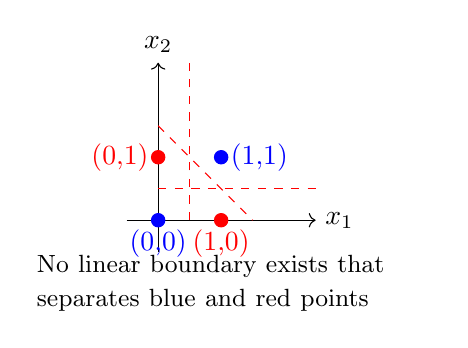
\begin{tikzpicture}[scale=0.8]
\draw[->] (-0.5,0) -- (2.5,0) node[right] {$x_1$};
\draw[->] (0,-0.5) -- (0,2.5) node[above] {$x_2$};

% XOR points
\filldraw[blue] (0,0) circle (3pt) node[below] {(0,0)};
\filldraw[red] (0,1) circle (3pt) node[left] {(0,1)};
\filldraw[red] (1,0) circle (3pt) node[below] {(1,0)};
\filldraw[blue] (1,1) circle (3pt) node[right] {(1,1)};

% Failed attempts
\draw[dashed,red] (0.5,0) -- (0.5,2.5);
\draw[dashed,red] (0,0.5) -- (2.5,0.5);
\draw[dashed,red] (0,1.5) -- (1.5,0);

\node[text width=5cm] at (1.2,-1) {
    \small{No linear boundary exists that separates blue and red points}
};
\end{tikzpicture}

\textbf{Historical Impact:}
\begin{itemize}
\item Minsky \& Papert (1969): \textit{Perceptrons} book
\item Led to first AI winter
\end{itemize}
\end{column}
\end{columns}
\end{frame}

\begin{frame}
\frametitle{Solving XOR with Logic Gates}

\textbf{Gate Combination:}
\begin{itemize}
\item OR Gate: $A + B$
\item NAND Gate: $\overline{A \cdot B}$ 
\item AND Gate: Combines previous outputs
\end{itemize}

\textbf{Boolean Expression:}
\[
XOR(A,B) = (A + B) \cdot \overline{A \cdot B}
\]
\[
= A\overline{B} + \overline{A}B
\]

\textbf{Circuit Analysis:}
\begin{enumerate}
\item OR gate detects any input activation
\item NAND gate detects non-simultaneous activation
\item AND gate ensures mutual exclusivity
\end{enumerate}

\end{frame}

\begin{frame}{How did we solve XOR using perceptron?}


\textbf{What we did right?}
\begin{itemize}
    \item<1-> Instead of single perceptron, we used multiple layers of perceptron (OR and NAND in layer 1 and AND in layer 2)
    \item<2-> We used non-linear (step function) transformation between layers
    \[
    \hat{y} = \begin{cases} 
    1 & \text{if } w_1x_1 + w_2x_2 \geq \theta \\
    0 & \text{otherwise}
    \end{cases}
    \]
    \item<3-> Most major milestones in Deep learning are because of
        \begin{itemize}
            \item increase the compute (mostly powered by hardware, trillion parameters -> today)
            \item Novel non-linearity between layers    
        \end{itemize}

\end{itemize}

\textbf{Where should we next?}
\begin{itemize}
    \item<3-> We used our domain knowledge in digital logic to design a perceptron for XOR
    \item<4-> We need to learn all the weights/parameters from data
\end{itemize}
    
\end{frame}




\subsection{Multi-Layer Perceptrons \& Backpropagation}
%%% 1980s: Backpropagation Breakthrough %%%
\begin{frame}
\frametitle{1980s: Backpropagation Revolution}

\textbf{Key Innovation:}
\begin{itemize}
\item \textbf{1986:} Rumelhart, Hinton \& Williams formalize backpropagation:
\begin{align*}
\delta^{(L)} &= (y - \hat{y}) \odot f'(z^{(L)}) \quad \text{(Output layer)} \\
\delta^{(l)} &= (W^{(l+1)T}\delta^{(l+1)}) \odot f'(z^{(l)}) \quad \text{(Hidden layers)}
\end{align*}
\end{itemize}

\begin{columns}[T]
\begin{column}{0.5\textwidth}
\textbf{Impact:}
\begin{itemize}
\item Enabled training of multi-layer networks`
\end{itemize}
\end{column}

\begin{column}{0.5\textwidth}
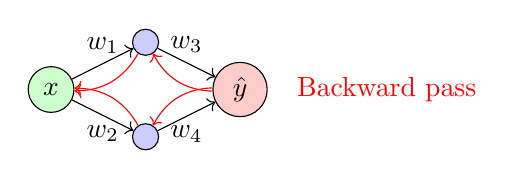
\begin{tikzpicture}[scale=0.6]
\node[draw,circle,fill=green!20] (x) at (0,0) {$x$};
\node[draw,circle,fill=blue!20] (h1) at (2,1) {};
\node[draw,circle,fill=blue!20] (h2) at (2,-1) {};
\node[draw,circle,fill=red!20] (y) at (4,0) {$\hat{y}$};

\draw[->] (x) -- (h1) node[midway,above] {$w_1$};
\draw[->] (x) -- (h2) node[midway,below] {$w_2$};
\draw[->] (h1) -- (y) node[midway,above] {$w_3$};
\draw[->] (h2) -- (y) node[midway,below] {$w_4$};

\draw[red,->] (y) edge[bend left] (h1);
\draw[red,->] (y) edge[bend right] (h2);
\draw[red,->] (h1) edge[bend left] (x);
\draw[red,->] (h2) edge[bend right] (x);
\node[red,right] at (5,0) {Backward pass};
\end{tikzpicture}
\end{column}
\end{columns}
\end{frame}

\begin{frame}
\frametitle{Backpropagation for XOR: Step-by-Step}

\begin{columns}[T]
\begin{column}{0.6\textwidth}
\textbf{Network Architecture:}
\begin{itemize}
\item Inputs: $x_1, x_2$ (XOR inputs)
\item Hidden Layer: 2 neurons (OR/NAND equivalents)
\item Output: 1 neuron (AND combination)
\item Activation: Sigmoid $\sigma(z) = \frac{1}{1+e^{-z}}$
\end{itemize}

\end{column}

\begin{column}{0.4\textwidth}
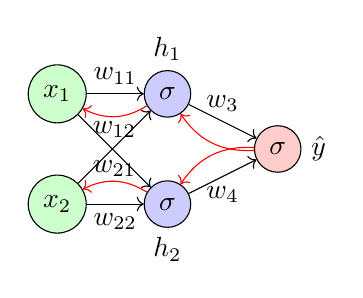
\begin{tikzpicture}[scale=0.7]
\node[draw,circle,fill=green!20] (x1) at (0,0) {$x_1$};
\node[draw,circle,fill=green!20] (x2) at (0,-2) {$x_2$};
\node[draw,circle,fill=blue!20,label=above:$h_1$] (h1) at (2,0) {$\sigma$};
\node[draw,circle,fill=blue!20,label=below:$h_2$] (h2) at (2,-2) {$\sigma$};
\node[draw,circle,fill=red!20,label=right:$\hat{y}$] (y) at (4,-1) {$\sigma$};

\draw[->] (x1) -- (h1) node[midway,above] {$w_{11}$};
\draw[->] (x1) -- (h2) node[midway,below] {$w_{21}$};
\draw[->] (x2) -- (h1) node[midway,above] {$w_{12}$};
\draw[->] (x2) -- (h2) node[midway,below] {$w_{22}$};
\draw[->] (h1) -- (y) node[midway,above] {$w_3$};
\draw[->] (h2) -- (y) node[midway,below] {$w_4$};

% Backprop arrows
\draw[red,->] (y) edge[bend left] (h1);
\draw[red,->] (y) edge[bend right] (h2);
\draw[red,->] (h1) edge[bend left] (x1);
\draw[red,->] (h2) edge[bend right] (x2);
\end{tikzpicture}
\end{column}
\end{columns}
\end{frame}

\begin{frame}
\frametitle{Backpropagation Mechanics for XOR Network}

\begin{columns}[T]
\begin{column}{0.6\textwidth}
\textbf{Network Structure:}
\begin{itemize}
\item \textbf{Input Layer:} $x_1, x_2$
\item \textbf{Hidden Layer:} $h_1, h_2$ with sigmoid $\sigma$
\item \textbf{Output Layer:} $\hat{y}$ with sigmoid $\sigma$
\end{itemize}

\textbf{Forward Propagation:}
\begin{align*}
z_1 &= w_{11}x_1 + w_{12}x_2 + b_1 \\
h_1 &= \sigma(z_1) \\
z_2 &= w_{21}x_1 + w_{22}x_2 + b_2 \\
h_2 &= \sigma(z_2) \\
z_3 &= w_3h_1 + w_4h_2 + b_3 \\
\hat{y} &= \sigma(z_3)
\end{align*}
\end{column}

\begin{column}{0.4\textwidth}
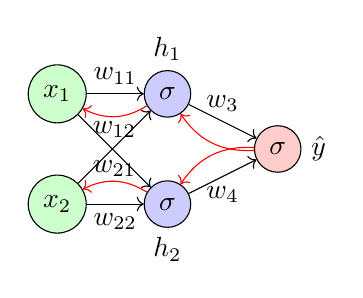
\begin{tikzpicture}[scale=0.7]
\node[draw,circle,fill=green!20] (x1) at (0,0) {$x_1$};
\node[draw,circle,fill=green!20] (x2) at (0,-2) {$x_2$};
\node[draw,circle,fill=blue!20,label=above:$h_1$] (h1) at (2,0) {$\sigma$};
\node[draw,circle,fill=blue!20,label=below:$h_2$] (h2) at (2,-2) {$\sigma$};
\node[draw,circle,fill=red!20,label=right:$\hat{y}$] (y) at (4,-1) {$\sigma$};

\draw[->] (x1) -- (h1) node[midway,above] {$w_{11}$};
\draw[->] (x1) -- (h2) node[midway,below] {$w_{21}$};
\draw[->] (x2) -- (h1) node[midway,above] {$w_{12}$};
\draw[->] (x2) -- (h2) node[midway,below] {$w_{22}$};
\draw[->] (h1) -- (y) node[midway,above] {$w_3$};
\draw[->] (h2) -- (y) node[midway,below] {$w_4$};

% Backprop arrows
\draw[red,->] (y) edge[bend left] (h1);
\draw[red,->] (y) edge[bend right] (h2);
\draw[red,->] (h1) edge[bend left] (x1);
\draw[red,->] (h2) edge[bend right] (x2);
\end{tikzpicture}
\end{column}
\end{columns}
\end{frame}

\subsection{Backpropagation Mechanics}
\begin{frame}
\frametitle{Gradient Computation Framework}

\textbf{Loss Function (MSE):}
\[
\mathcal{L} = \frac{1}{2}(y - \hat{y})^2
\]

\textbf{Chain Rule Decomposition:}
\begin{align*}
\frac{\partial \mathcal{L}}{\partial w_3} &= \underbrace{(y - \hat{y})}_{\text{Error}} \cdot \underbrace{\hat{y}(1-\hat{y})}_{\sigma'} \cdot h_1 \\
\frac{\partial \mathcal{L}}{\partial w_{11}} &= \frac{\partial \mathcal{L}}{\partial h_1} \cdot \frac{\partial h_1}{\partial z_1} \cdot x_1 
\end{align*}
\end{frame}

\begin{frame}
\frametitle{Computing Hidden Layer Gradients}

\textbf{Chain Rule for $w_{11}$:}
\begin{align*}
\frac{\partial \mathcal{L}}{\partial w_{11}} &= 
\underbrace{\frac{\partial \mathcal{L}}{\partial \hat{y}}}_{\text{Output Error}} 
\cdot \underbrace{\frac{\partial \hat{y}}{\partial z_3}}_{\text{Output Activation}} 
\cdot \underbrace{\frac{\partial z_3}{\partial h_1}}_{\text{Output Weight}} 
\cdot \underbrace{\frac{\partial h_1}{\partial z_1}}_{\text{Hidden Activation}} 
\cdot \underbrace{\frac{\partial z_1}{\partial w_{11}}}_{\text{Input Value}} \\
&= (y - \hat{y}) \cdot \hat{y}(1-\hat{y}) \cdot w_3 \cdot h_1(1-h_1) \cdot x_1
\end{align*}

\textbf{Component Explanation for $w_{11}$:}
{\footnotesize
\begin{itemize}
\item $\frac{\partial \mathcal{L}}{\partial \hat{y}} = \frac{\partial}{\partial \hat{y}} [\frac{1}{2}(y - \hat{y})^2] = (y - \hat{y})$: Direct error measurement
\item $\frac{\partial \hat{y}}{\partial z_3} = \frac{\partial}{\partial z_3} \sigma(z_3) = \hat{y}(1-\hat{y})$: Output activation derivative
\item $\frac{\partial z_3}{\partial h_1} = \frac{\partial}{\partial h_1} (w_3h_1 + w_4h_2 + b_3) = w_3$: Output weight contribution
\item $\frac{\partial h_1}{\partial z_1} = \frac{\partial}{\partial z_1} \sigma(z_1) = h_1(1-h_1)$: Hidden activation derivative
\item $\frac{\partial z_1}{\partial w_{11}} = \frac{\partial}{\partial w_{11}} (w_{11}x_1 + w_{12}x_2 + b_1) = x_1$: Input contribution
\end{itemize}
}

\end{frame}

\begin{frame}
\frametitle{Updating Parameters: The Optimization Step}

\textbf{The Weight Update Rule:}
After computing the gradients using backpropagation, we adjust each parameter to minimize the loss function $\mathcal{L}$.

\textbf{General Gradient Descent Formula:}
\[
w \leftarrow w - \eta \cdot \frac{\partial \mathcal{L}}{\partial w}
\]

\textbf{Application to $w_{11}$:}
Substituting our derived chain rule result:
\[
w_{11} \leftarrow w_{11} + \eta \cdot \underbrace{\left[ (y - \hat{y}) \cdot \hat{y}(1-\hat{y}) \cdot w_3 \cdot h_1(1-h_1) \cdot x_1 \right]}_{\text{Error Signal Propagation}}
\]

\end{frame}

\begin{frame}
\frametitle{Global Parameter Updates for XOR Network}

{\footnotesize
\textbf{Output Layer Weights (2 neurons):}
\begin{align*}
w_3 &\leftarrow w_3 + \eta \cdot (y - \hat{y}) \cdot \hat{y}(1-\hat{y}) \cdot h_1 \\
w_4 &\leftarrow w_4 + \eta \cdot (y - \hat{y}) \cdot \hat{y}(1-\hat{y}) \cdot h_2
\end{align*}

\textbf{Hidden Layer Weights (4 links):}
\begin{align*}
w_{11} &\leftarrow w_{11} + \eta \cdot (y - \hat{y}) \cdot \hat{y}(1-\hat{y}) \cdot w_3 \cdot h_1(1-h_1) \cdot x_1 \\
w_{12} &\leftarrow w_{12} + \eta \cdot (y - \hat{y}) \cdot \hat{y}(1-\hat{y}) \cdot w_3 \cdot h_1(1-h_1) \cdot x_2 \\
w_{21} &\leftarrow w_{21} + \eta \cdot (y - \hat{y}) \cdot \hat{y}(1-\hat{y}) \cdot w_4 \cdot h_2(1-h_2) \cdot x_1 \\
w_{22} &\leftarrow w_{22} + \eta \cdot (y - \hat{y}) \cdot \hat{y}(1-\hat{y}) \cdot w_4 \cdot h_2(1-h_2) \cdot x_2
\end{align*}
}

\vfill
{\footnotesize
\textit{Derivation for one of these weights could be a question in the exam.} \\
(Follow the same chain rule principles used for $w_{11}$ on the previous slide.)
}
\end{frame}


\begin{frame}
\frametitle{Why Subtract the Gradient? The Intuition}

\begin{columns}[T]
\begin{column}{0.6\textwidth}
\textbf{Understanding the Direction:}
The derivative $\frac{\partial \mathcal{L}}{\partial w}$ represents the \textbf{slope} of the loss function. It tells us how the loss changes if we increase the weight $w$.

\begin{itemize}
    \item \textbf{Scenario 1: Positive Slope}
    \begin{itemize}
        \item Increasing $w$ \textbf{increases} the loss.
        \item To minimize, we \textbf{decrease} $w$. 
    \end{itemize}
    \item \textbf{Scenario 2: Negative Slope}
    \begin{itemize}
        \item Increasing $w$ \textbf{decreases} the loss.
        \item To minimize, we \textbf{increase} $w$.
    \end{itemize}
\end{itemize}

\textbf{Universal Rule:}
Subtracting the gradient always moves us \textbf{opposite} to the uphill direction.

And hence the name \textbf{Gradient Descent}
\end{column}

\begin{column}{0.35\textwidth}
\centering
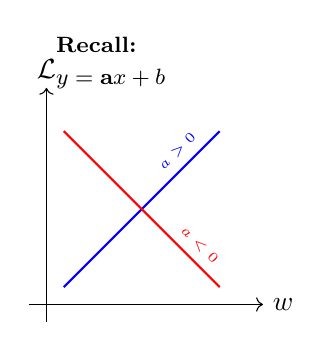
\begin{tikzpicture}[scale=1.1]
    \draw[->] (-0.2,0) -- (2.5,0) node[right] {$w$};
    \draw[->] (0,-0.2) -- (0,2.5) node[above] {$\mathcal{L}$};
    
    % Recall note
    \node[anchor=west] at (0,3.0) {\footnotesize \textbf{Recall:}};
    \node[anchor=west] at (0,2.6) {\footnotesize $y = \mathbf{a}x + b$};
    
    % Positive Slope
    \draw[blue, thick] (0.2,0.2) -- (2.0,2.0) node[pos=0.8, sloped, above] {\tiny $a > 0$};
    
    % Negative Slope
    \draw[red, thick] (0.2,2.0) -- (2.0,0.2) node[pos=0.8, sloped, above] {\tiny $a < 0$};
\end{tikzpicture}
\end{column}
\end{columns}

\end{frame}

\begin{frame}
\frametitle{Update Rule: Key Concepts}

\begin{itemize}
    \item \textbf{Learning Rate ($\eta$):} A small positive scalar (e.g., $0.01$) that controls the weight adjustment step size.
    \begin{itemize}
        \item Too large $\to$ oscillation or divergence.
        \item Too small $\to$ slow convergence.
    \end{itemize}
    \item \textbf{Global Update:} This process is repeated for \textit{every} weight ($w_{ij}$) and bias ($b_i$) in the network.
    \item \textbf{Iteration (Epoch):} One full pass through the entire training dataset is called an \textbf{Epoch}. Training usually requires hundreds or thousands of epochs to converge.
\end{itemize}

\end{frame}


\section{Scaling Deep Learning: Vectorization}
\subsection{Matrix Math \& Batching}
\begin{frame}{Parallel Forward and Backward computation}
\centering
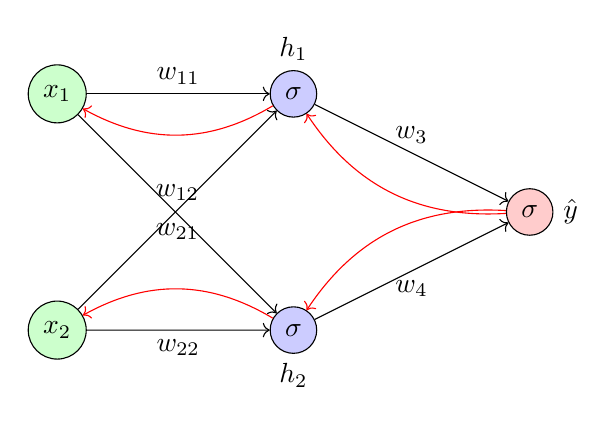
\begin{tikzpicture}[scale=1.5]
\node[draw,circle,fill=green!20] (x1) at (0,0) {$x_1$};
\node[draw,circle,fill=green!20] (x2) at (0,-2) {$x_2$};
\node[draw,circle,fill=blue!20,label=above:$h_1$] (h1) at (2,0) {$\sigma$};
\node[draw,circle,fill=blue!20,label=below:$h_2$] (h2) at (2,-2) {$\sigma$};
\node[draw,circle,fill=red!20,label=right:$\hat{y}$] (y) at (4,-1) {$\sigma$};

\draw[->] (x1) -- (h1) node[midway,above] {$w_{11}$};
\draw[->] (x1) -- (h2) node[midway,below] {$w_{21}$};
\draw[->] (x2) -- (h1) node[midway,above] {$w_{12}$};
\draw[->] (x2) -- (h2) node[midway,below] {$w_{22}$};
\draw[->] (h1) -- (y) node[midway,above] {$w_3$};
\draw[->] (h2) -- (y) node[midway,below] {$w_4$};

% Backprop arrows
\draw[red,->] (y) edge[bend left] (h1);
\draw[red,->] (y) edge[bend right] (h2);
\draw[red,->] (h1) edge[bend left] (x1);
\draw[red,->] (h2) edge[bend right] (x2);
\end{tikzpicture}
    
\end{frame}

\begin{frame}{Batch Forward Pass: From Vectors to Matrices}
To process a batch of size $B$, we stack individual input vectors into a matrix $X$. This allows us to leverage highly optimized Matrix-Matrix multiplication (GEMM) on hardware like GPUs.

\begin{columns}[T]
\begin{column}{0.45\textwidth}
\textbf{Individual Example:}
{\footnotesize
\[ z^{(i)}_h = x^{(i)} W_h + b_h \]
\[ h^{(i)} = \sigma(z^{(i)}_h) \]
}
\end{column}
\begin{column}{0.5\textwidth}
\textbf{Batch Computation:}
{\footnotesize
\[ \underbrace{Z_h}_{B \times 2} = \underbrace{X}_{B \times 2} \underbrace{W_h}_{2 \times 2} + \underbrace{b_h}_{1 \times 2} \]
\[ \underbrace{H}_{B \times 2} = \sigma(Z_h) \]
}
\end{column}
\end{columns}

\vspace{0.8cm}
\textbf{Final Prediction for Batch:}
\[ \underbrace{\hat{Y}}_{B \times 1} = \sigma \left( \underbrace{H}_{B \times 2} \underbrace{W_o}_{2 \times 1} + \underbrace{b_o}_{1 \times 1} \right) \]

\centering
\textit{Computationally efficient: One large matrix operation is much faster than $B$ small vector operations.}
\end{frame}

\begin{frame}{Matrix Anatomy: XOR Batch (B=4)}
\begin{columns}[T]
\begin{column}{0.48\textwidth}
\textbf{1. Matrix $X$ (Inputs):} \\
Each \textbf{row} is a different training sample.
\[ X = \begin{bmatrix} 0 & 0 \\ 0 & 1 \\ 1 & 0 \\ 1 & 1 \end{bmatrix} \in \mathbb{R}^{4 \times 2} \]

\textbf{2. Matrix $W_h$ (Weights):} \\
Each \textbf{column} leads to one hidden neuron.
\[ W_h = \begin{bmatrix} w_{11} & w_{21} \\ w_{12} & w_{22} \end{bmatrix} \in \mathbb{R}^{2 \times 2} \]
{\tiny $\leftarrow$ row 1: from $x_1$, row 2: from $x_2$}
\end{column}

\begin{column}{0.48\textwidth}
\textbf{3. Matrix $H$ (Hidden States):} \\
Result of the entire batch forward pass: $H = \sigma(X W_h + b_h)$
\[ H = \begin{bmatrix} h_1^{(0,0)} & h_2^{(0,0)} \\ h_1^{(0,1)} & h_2^{(0,1)} \\ h_1^{(1,0)} & h_2^{(1,0)} \\ h_1^{(1,1)} & h_2^{(1,1)} \end{bmatrix} \in \mathbb{R}^{4 \times 2} \]
\end{column}
\end{columns}

\vfill
\centering
\textbf{Logic:} Batch processing converts many small \textit{spatial} computations into one large \textit{structural} computation.
\end{frame}


\subsection{Vectorized Batch Gradients}
\begin{frame}{The Goal: Efficient Batch Gradients}
How do we calculate the average gradient for $B$ examples without using a slow \texttt{for} loop?

\textbf{The Mathematical Challenge:}
The global update requires the average of gradients from every example in the batch:
\[ \frac{\partial \mathcal{L}_{\text{total}}}{\partial W} = \frac{1}{B} \sum_{i=1}^{B} \nabla W^{(i)} \]

\textbf{The Vectorized Solution:}
Instead of $B$ separate operations, we use \textbf{Matrix Transpose Multiplication}.
\begin{itemize}
    \item \textbf{Loop-based:} $O(B)$ sequential vector operations.
    \item \textbf{Matrix form:} A single call to optimized GPU kernels (CUDA/cuBLAS) that process all examples in parallel.
\end{itemize}
\end{frame}

\begin{frame}{Defining the Error Signal $\delta_o$}
The term \textbf{$\delta$} (Delta) is fundamental to backpropagation. It represents the \textbf{sensitivity of the loss to the pre-activation ($Z$)}.

\textbf{Formal Definition (Output Layer):}
\[ \delta_o = \frac{\partial \mathcal{L}}{\partial Z_o} \]

\textbf{Backpropagation Logic:}
To compute $\delta_o$, we use the chain rule to combine how the loss changes with the prediction ($\hat{Y}$) and how the prediction changes with the pre-activation ($Z_o$):
\[ 
\delta_o = \underbrace{\frac{\partial \mathcal{L}}{\partial \hat{Y}}}_{\text{Rate of Error Change}} \odot \underbrace{\frac{\partial \hat{Y}}{\partial Z_o}}_{\text{Activation Slope}} 
\]

\vfill
\centering
\textit{This term acts as the "error signal" that gets passed backward through the gates.}
\end{frame}

\begin{frame}{Step 1: The Batch Error Signal ($\delta_o$)}
First, we stack the individual error signals into a single "Error Matrix".

\textbf{Matrix Formulation:}
Calculating the difference between predictions and targets for the whole batch:
\[ \underbrace{\delta_o}_{B \times 1} = \underbrace{(\hat{Y} - Y)}_{\substack{\text{Output Error} \\ (B \times 1)}} \odot \underbrace{\sigma'(Z_o)}_{\substack{\text{Output Activation} \\ (B \times 1)}} \]

\textbf{What's inside?}
\[ \underbrace{\begin{bmatrix} \delta_o^{(1)} \\ \vdots \\ \delta_o^{(B)} \end{bmatrix}}_{\delta_o} = \underbrace{\begin{bmatrix} \hat{y}^{(1)} - y^{(1)} \\ \vdots \\ \hat{y}^{(B)} - y^{(B)} \end{bmatrix}}_{\text{Error Vector}} \odot \underbrace{\begin{bmatrix} \sigma'(z_o^{(1)}) \\ \vdots \\ \sigma'(z_o^{(B)}) \end{bmatrix}}_{\text{Activation Slope}} \]
Each row in this matrix "captures" the specific error contribution of one training sample.
\end{frame}

\begin{frame}{Defining Weight Gradients: $\frac{\partial \mathcal{L}}{\partial W_o}$}
Once we have calculated the error signal $\delta_o$, we can determine how the output weights $W_o$ contributed to that error.

\textbf{Backpropagation (Weight Update):}
The weight $W_o$ affects the loss only through the pre-activation $Z_o$:
\[ 
\frac{\partial \mathcal{L}}{\partial W_o} = \underbrace{\frac{\partial \mathcal{L}}{\partial Z_o}}_{\text{Error Signal } (\delta_o)} \cdot \underbrace{\frac{\partial Z_o}{\partial W_o}}_{\text{Value of Activation } (H)} 
\]

\textbf{The Matrix Derivative Rule:}
By applying the standard matrix calculus rule for the linear relationship $Z_o = H W_o + b_o$, our activation matrix is transposed to align dimensions:
\[ 
\nabla W_o = \frac{\partial \mathcal{L}}{\partial W_o} = \mathbf{\frac{1}{B} H^T \delta_o}
\]

\vfill
\centering
\textit{This transpose operation efficiently sums the gradients for all $B$ samples into a single parameter update.}
\end{frame}

\begin{frame}{Step 2: Propagating to Hidden Layers}
To compute the hidden weights $W_h$, we first "push" the error back from the output layer to see how $H$ contributed to the final result.

\textbf{1. The Hidden Error Signal ($\delta_h$):}
By applying the matrix derivative rule to the linear relationship $Z_o = H W_o + b_o$, we find $\frac{\partial \mathcal{L}}{\partial H} = \delta_o W_o^T$.
\[ 
\underbrace{\delta_h}_{B \times 2} = \frac{\partial \mathcal{L}}{\partial Z_h} = \underbrace{\frac{\partial \mathcal{L}}{\partial Z_o}}_{\delta_o} \underbrace{\frac{\partial Z_o}{\partial H}}_{W_{o}^T}  \underbrace{\frac{\partial H}{\partial Z_h}}_{\sigma'(Z_h)} = (\delta_o W_o^T) \odot \sigma'(Z_h)
\]

\textbf{2. Final Gradient for Hidden Weights ($W_h$):}
Using the same matrix derivation rule as the output layer:
\[ 
\underbrace{\nabla W_h}_{2 \times 2} = \frac{\partial \mathcal{L}}{\partial W_h} = \mathbf{\frac{1}{B} X^T \delta_h}
\]

\vfill
\centering
\textbf{Conclusion:} One massive "structural" pass handles the entire batch at once using just matrix algebra!
\end{frame}


\subsection{Hands-On: Perceptron \& XOR}
\begin{frame}{Hands-On Session}
\begin{figure}
    \centering
    
\includegraphics[width=0.3\linewidth]{images/image2.png}
\end{figure}

\begin{itemize}
    \item Click here to download/open the notebook: \attachfile[color=0.5 0.5 0.5]{hands-on/Perceptron_Hands_ON.ipynb} (or click \href{run:hands-on/Perceptron_Hands_ON.ipynb}{here} to open if supported)
\end{itemize}



% gates = {
%     'or_gate': Perceptron(weights=np.array([0.5, 0.5]), threshold=0.3),
%     'nand_gate': Perceptron(weights=np.array([-0.5, -0.5]), threshold=-0.7),
%     'and_gate': Perceptron(weights=np.array([0.5, 0.5]), threshold=0.7)
%     }
    
\end{frame}

%% Slide 7: History of Deep Learning
\begin{frame}
\frametitle{Brief History of Deep Learning}
\begin{itemize}
    \item 1940s-50s: McCulloch, Pitts, and Rosenblatt develop perceptron
    \item 1980s: Backpropagation algorithm formalized
    \textbf{
    \item 1990s: LeCun develops LeNet for digit recognition
    \item 2012: AlexNet wins ImageNet competition
    }
    \item 2014-present: Explosion of deep learning research and applications
\end{itemize}
\end{frame}


\section{Key Components \& Architectures}
\subsection{Neural Network Fundamentals}
%% Slide 9: What is a Neural Network?
\begin{frame}
\frametitle{What is a Neural Network?}
\begin{itemize}
    \item Computational system inspired by biological neural networks
    \item Composed of interconnected nodes (``neurons'')
    \item Learns to perform tasks by analyzing examples
    \item Excels at finding patterns in complex, high-dimensional data
    \item Universal function approximators (can theoretically learn any function)
\end{itemize}
\end{frame}

%% Slide 10: Neural Network Components
\begin{frame}
\frametitle{Neural Network Components}
\begin{itemize}
    \item \textbf{Neurons:} Computational units that process inputs
    \item \textbf{Weights:} Parameters determining input importance
    \item \textbf{Bias:} Additional parameter for flexibility
    \item \textbf{Activation Functions:} Non-linear transformations (ReLU, sigmoid, tanh)
    \item \textbf{Layers:} Collections of neurons
    \begin{itemize}
        \item Input layer
        \item Hidden layer(s)
        \item Output layer
    \end{itemize}
\end{itemize}
\end{frame}

\subsection{Activation Functions}
%% Slide 11: Activation Functions
\begin{frame}
\frametitle{Common Activation Functions}
\begin{itemize}
    \item \textbf{Sigmoid:} $\sigma(x) = \frac{1}{1+e^{-x}}$
    \begin{itemize}
        \item Output range [0,1], historically common
    \end{itemize}
    \item \textbf{Tanh:} $\tanh(x) = \frac{e^x - e^{-x}}{e^x + e^{-x}}$
    \begin{itemize}
        \item Output range [-1,1], zero-centered
    \end{itemize}
    \item \textbf{ReLU:} $f(x) = \max(0,x)$
    \begin{itemize}
        \item Sparse activation, reduces vanishing gradient
    \end{itemize}
    \item \textbf{Leaky ReLU:} $f(x) = \max(\alpha x,x)$ where $\alpha$ is small
    \begin{itemize}
        \item Addresses dying ReLU problem
    \end{itemize}
    \item \textbf{Softmax:} For multi-class outputs, normalizes to probability distribution
\end{itemize}
\end{frame}

%% Slide 12: Feedforward Neural Networks
\begin{frame}
\frametitle{Feedforward Neural Networks}
\begin{columns}
\begin{column}{0.48\textwidth}
\begin{itemize}
    \item Simplest architecture, information flows in one direction
    \item Also called Multi-Layer Perceptrons (MLPs)
    \item Each neuron connected to all neurons in adjacent layers
    \item No connections between neurons in the same layer
    \item Universal function approximators
    \item Limited in handling structured data (images, sequences)
\end{itemize}
\end{column}
\begin{column}{0.48\textwidth}
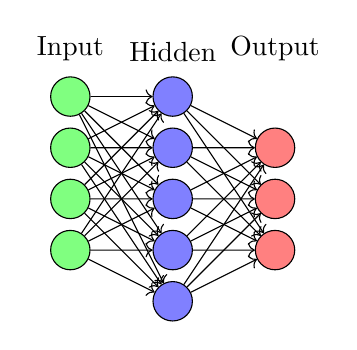
\begin{tikzpicture}[scale=0.65]
    % Define node styles
    \tikzstyle{neuron}=[circle, draw, minimum size=0.5cm]
    \tikzstyle{input neuron}=[neuron, fill=green!50]
    \tikzstyle{hidden neuron}=[neuron, fill=blue!50]
    \tikzstyle{output neuron}=[neuron, fill=red!50]
    
    % Draw input layer
    \foreach \i in {1,...,4} {
        \node[input neuron] (I-\i) at (0,-\i) {};
    }
    
    % Draw hidden layer
    \foreach \i in {1,...,5} {
        \node[hidden neuron] (H-\i) at (2,-\i) {};
    }
    
    % Draw output layer
    \foreach \i in {1,...,3} {
        \node[output neuron] (O-\i) at (4,-\i-1) {};
    }
    
    % Connect layers
    \foreach \i in {1,...,4} {
        \foreach \j in {1,...,5} {
            \draw[->] (I-\i) -- (H-\j);
        }
    }
    
    \foreach \i in {1,...,5} {
        \foreach \j in {1,...,3} {
            \draw[->] (H-\i) -- (O-\j);
        }
    }
    
    % Labels
    \node[anchor=south] at (0,-0.5) {Input};
    \node[anchor=south] at (2,-0.5) {Hidden};
    \node[anchor=south] at (4,-0.5) {Output};
\end{tikzpicture}
\end{column}
\end{columns}
\end{frame}

\subsection{Convolutional Neural Networks (CNNs)}
%% Slide 13: Convolutional Neural Networks (CNNs)
\begin{frame}
\frametitle{Convolutional Neural Networks (CNNs)}
\begin{itemize}
    \item Specialized for processing grid-like data (images)
    \item Key operations:
    \begin{itemize}
        \item \textbf{Convolution:} Filters detect local patterns
        \item \textbf{Pooling:} Reduces dimensionality, provides translation invariance
        \item \textbf{Fully connected layers:} Final classification/regression
    \end{itemize}
    \item Hierarchical feature learning:
    \begin{itemize}
        \item Early layers: Edges, textures
        \item Middle layers: Shapes, parts
        \item Deeper layers: Objects, concepts
    \end{itemize}
\end{itemize}
\end{frame}

%% Slide 14: CNN Architecture Example
\begin{frame}
\frametitle{CNN Architecture Example}
\begin{center}
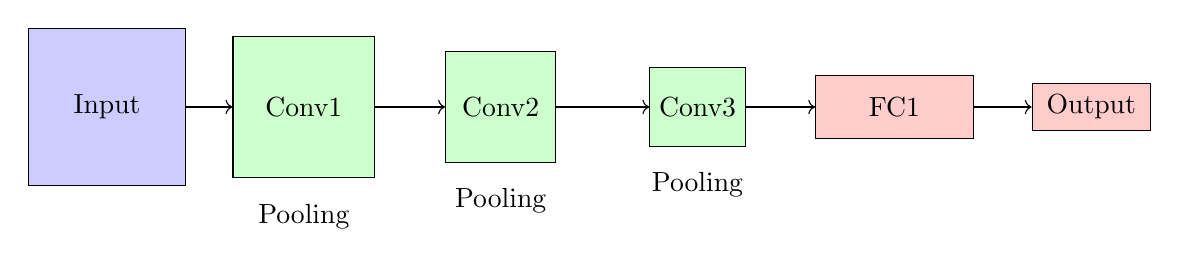
\begin{tikzpicture}[scale=0.5]
    % Input image
    \node[rectangle, minimum size=2cm, draw, fill=blue!20] (input) at (-2,0) {Input};
    
    % Convolutional layers
    \node[rectangle, minimum height=1.8cm, minimum width=1.8cm, draw, fill=green!20] (conv1) at (3,0) {Conv1};
    
    \node[rectangle, minimum height=1.4cm, minimum width=1.4cm, draw, fill=green!20] (conv2) at (8,0) {Conv2};
    
    \node[rectangle, minimum height=1cm, minimum width=1cm, draw, fill=green!20] (conv3) at (13,0) {Conv3};
    
    % Fully connected layers
    \node[rectangle, minimum height=0.8cm, minimum width=2cm, draw, fill=red!20] (fc1) at (18,0) {FC1};
    
    % Output layer
    \node[rectangle, minimum height=0.6cm, minimum width=1.5cm, draw, fill=red!20] (output) at (23,0) {Output};
    
    % Connections
    \draw[->] (input) -- (conv1);
    \draw[->] (conv1) -- (conv2);
    \draw[->] (conv2) -- (conv3);
    \draw[->] (conv3) -- (fc1);
    \draw[->] (fc1) -- (output);
    
    % Pooling operations
    \node[below=0.2cm of conv1] {Pooling};
    \node[below=0.2cm of conv2] {Pooling};
    \node[below=0.2cm of conv3] {Pooling};
\end{tikzpicture}
\end{center}

Key innovations:
\begin{itemize}
    \item Local receptive fields
    \item Parameter sharing
    \item Hierarchical feature extraction
\end{itemize}
\end{frame}


%% Slide 3: The Convolution Operation
\begin{frame}
\frametitle{Convolution Operation: The Core Mechanism}

\begin{columns}
\begin{column}{0.5\textwidth}
\textbf{Key Idea:}
\begin{itemize}
\item Slide a filter/kernel across input
\item Compute element-wise products
\item Sum products to create feature maps
\end{itemize}

\textbf{Mathematical Form:}
For 2D: 
\[ (I * K)[i,j] = \sum_{m}\sum_{n} I[i+m,j+n] \cdot K[m,n] \]

\end{column}

\begin{column}{0.5\textwidth}
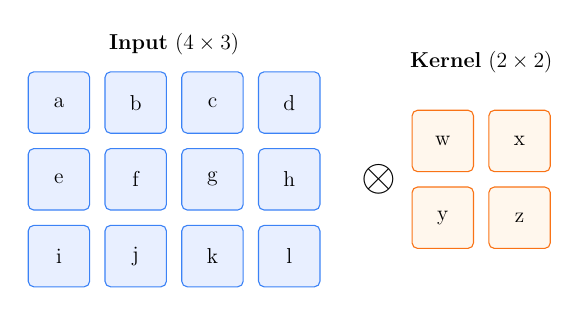
\begin{tikzpicture}[scale=0.65, every node/.style={transform shape}]
    % Palette
    \definecolor{inputColor}{HTML}{E8EFFF}
    \definecolor{inputBorder}{HTML}{3B82F6}
    \definecolor{kernelColor}{HTML}{FFF7ED}
    \definecolor{kernelBorder}{HTML}{F97316}

    % --- Input Matrix ---
    \begin{scope}[shift={(0,0)}]
        \node[above] at (2.25, 0.8) {\large \textbf{Input} ($4 \times 3$)};
        
        \node[draw=inputBorder, fill=inputColor, minimum size=1.2cm, rounded corners=2pt, font=\large] (a) at (0,0) {a};
        \node[draw=inputBorder, fill=inputColor, minimum size=1.2cm, rounded corners=2pt, font=\large] (b) at (1.5,0) {b};
        \node[draw=inputBorder, fill=inputColor, minimum size=1.2cm, rounded corners=2pt, font=\large] (c) at (3,0) {c};
        \node[draw=inputBorder, fill=inputColor, minimum size=1.2cm, rounded corners=2pt, font=\large] (d) at (4.5,0) {d};
        
        \node[draw=inputBorder, fill=inputColor, minimum size=1.2cm, rounded corners=2pt, font=\large] (e) at (0,-1.5) {e};
        \node[draw=inputBorder, fill=inputColor, minimum size=1.2cm, rounded corners=2pt, font=\large] (f) at (1.5,-1.5) {f};
        \node[draw=inputBorder, fill=inputColor, minimum size=1.2cm, rounded corners=2pt, font=\large] (g) at (3,-1.5) {g};
        \node[draw=inputBorder, fill=inputColor, minimum size=1.2cm, rounded corners=2pt, font=\large] (h) at (4.5,-1.5) {h};
        
        \node[draw=inputBorder, fill=inputColor, minimum size=1.2cm, rounded corners=2pt, font=\large] (i) at (0,-3) {i};
        \node[draw=inputBorder, fill=inputColor, minimum size=1.2cm, rounded corners=2pt, font=\large] (j) at (1.5,-3) {j};
        \node[draw=inputBorder, fill=inputColor, minimum size=1.2cm, rounded corners=2pt, font=\large] (k) at (3,-3) {k};
        \node[draw=inputBorder, fill=inputColor, minimum size=1.2cm, rounded corners=2pt, font=\large] (l) at (4.5,-3) {l};
    \end{scope}

    % Op Symbol
    \node at (6.25, -1.5) {\Huge $\otimes$};

    % --- Kernel ---
    \begin{scope}[shift={(7.5, -0.75)}]
        \node[above] at (0.75, 1.2) {\large \textbf{Kernel} ($2 \times 2$)};
        \node[draw=kernelBorder, fill=kernelColor, minimum size=1.2cm, rounded corners=2pt, font=\large] (w) at (0,0) {w};
        \node[draw=kernelBorder, fill=kernelColor, minimum size=1.2cm, rounded corners=2pt, font=\large] (x) at (1.5,0) {x};
        \node[draw=kernelBorder, fill=kernelColor, minimum size=1.2cm, rounded corners=2pt, font=\large] (y) at (0,-1.5) {y};
        \node[draw=kernelBorder, fill=kernelColor, minimum size=1.2cm, rounded corners=2pt, font=\large] (z) at (1.5,-1.5) {z};
    \end{scope}

\end{tikzpicture}
\end{column}
\end{columns}

\end{frame}

%% Slide 4: Convolution Visualization
\begin{frame}
\frametitle{Convolution in Action (Stride 1)}

\begin{center}
    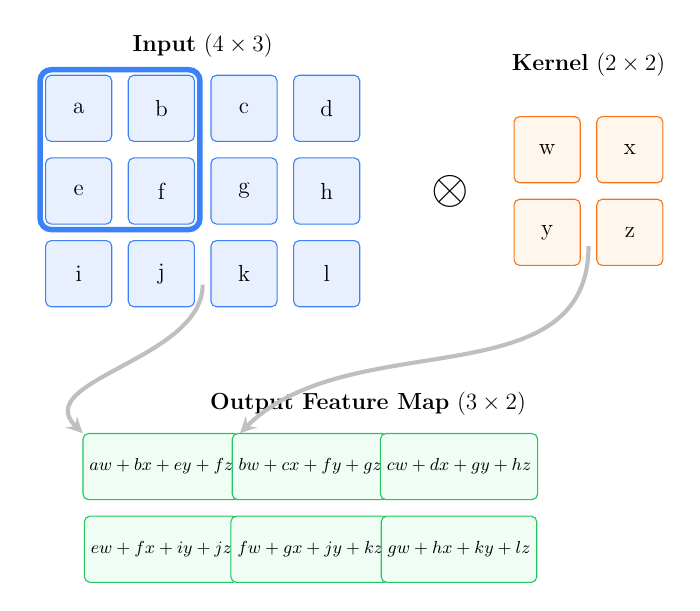
\begin{tikzpicture}[scale=0.7, every node/.style={transform shape}]
    % Color Palette
    \definecolor{inputColor}{HTML}{E8EFFF}
    \definecolor{inputBorder}{HTML}{3B82F6}
    \definecolor{kernelColor}{HTML}{FFF7ED}
    \definecolor{kernelBorder}{HTML}{F97316}
    \definecolor{outputColor}{HTML}{F0FDF4}
    \definecolor{outputBorder}{HTML}{22C55E}
    
    % --- Input Matrix (Top Left) ---
    \begin{scope}[shift={(0,0)}]
        \node[above] at (2.25, 0.8) {\large \textbf{Input} ($4 \times 3$)};
        
        \node[draw=inputBorder, fill=inputColor, minimum size=1.2cm, rounded corners=2pt, font=\large] (a) at (0,0) {a};
        \node[draw=inputBorder, fill=inputColor, minimum size=1.2cm, rounded corners=2pt, font=\large] (b) at (1.5,0) {b};
        \node[draw=inputBorder, fill=inputColor, minimum size=1.2cm, rounded corners=2pt, font=\large] (c) at (3,0) {c};
        \node[draw=inputBorder, fill=inputColor, minimum size=1.2cm, rounded corners=2pt, font=\large] (d) at (4.5,0) {d};
        
        \node[draw=inputBorder, fill=inputColor, minimum size=1.2cm, rounded corners=2pt, font=\large] (e) at (0,-1.5) {e};
        \node[draw=inputBorder, fill=inputColor, minimum size=1.2cm, rounded corners=2pt, font=\large] (f) at (1.5,-1.5) {f};
        \node[draw=inputBorder, fill=inputColor, minimum size=1.2cm, rounded corners=2pt, font=\large] (g) at (3,-1.5) {g};
        \node[draw=inputBorder, fill=inputColor, minimum size=1.2cm, rounded corners=2pt, font=\large] (h) at (4.5,-1.5) {h};
        
        \node[draw=inputBorder, fill=inputColor, minimum size=1.2cm, rounded corners=2pt, font=\large] (i) at (0,-3) {i};
        \node[draw=inputBorder, fill=inputColor, minimum size=1.2cm, rounded corners=2pt, font=\large] (j) at (1.5,-3) {j};
        \node[draw=inputBorder, fill=inputColor, minimum size=1.2cm, rounded corners=2pt, font=\large] (k) at (3,-3) {k};
        \node[draw=inputBorder, fill=inputColor, minimum size=1.2cm, rounded corners=2pt, font=\large] (l) at (4.5,-3) {l};
    \end{scope}

    % Highlight first position
    \draw[inputBorder, line width=2pt, rounded corners=4pt] (-0.7,0.7) rectangle (2.2,-2.2);

    % --- Kernel (Top Right) ---
    \begin{scope}[shift={(8.5, -0.75)}]
        \node[above] at (0.75, 1.2) {\large \textbf{Kernel} ($2 \times 2$)};
        \node[draw=kernelBorder, fill=kernelColor, minimum size=1.2cm, rounded corners=2pt, font=\large] (w) at (0,0) {w};
        \node[draw=kernelBorder, fill=kernelColor, minimum size=1.2cm, rounded corners=2pt, font=\large] (x) at (1.5,0) {x};
        \node[draw=kernelBorder, fill=kernelColor, minimum size=1.2cm, rounded corners=2pt, font=\large] (y) at (0,-1.5) {y};
        \node[draw=kernelBorder, fill=kernelColor, minimum size=1.2cm, rounded corners=2pt, font=\large] (z) at (1.5,-1.5) {z};
    \end{scope}

    % Mathematical Symbol
    \node at (6.75, -1.5) {\Huge $\otimes$};

    % --- Output Matrix (Bottom) ---
    \begin{scope}[shift={(1.5, -6.5)}]
        \node[above] at (3.75, 0.8) {\large \textbf{Output Feature Map} ($3 \times 2$)};
        
        \node[draw=outputBorder, fill=outputColor, minimum width=2.5cm, minimum height=1.2cm, rounded corners=2pt, font=\small] (o1) at (0,0) {$aw+bx+ey+fz$};
        \node[draw=outputBorder, fill=outputColor, minimum width=2.5cm, minimum height=1.2cm, rounded corners=2pt, font=\small] (o2) at (2.7,0) {$bw+cx+fy+gz$};
        \node[draw=outputBorder, fill=outputColor, minimum width=2.5cm, minimum height=1.2cm, rounded corners=2pt, font=\small] (o3) at (5.4,0) {$cw+dx+gy+hz$};
        
        \node[draw=outputBorder, fill=outputColor, minimum width=2.5cm, minimum height=1.2cm, rounded corners=2pt, font=\small] (o4) at (0,-1.5) {$ew+fx+iy+jz$};
        \node[draw=outputBorder, fill=outputColor, minimum width=2.5cm, minimum height=1.2cm, rounded corners=2pt, font=\small] (o5) at (2.7,-1.5) {$fw+gx+jy+kz$};
        \node[draw=outputBorder, fill=outputColor, minimum width=2.5cm, minimum height=1.2cm, rounded corners=2pt, font=\small] (o6) at (5.4,-1.5) {$gw+hx+ky+lz$};
    \end{scope}

    % Arrows connecting to output
    \draw[->, >=stealth, line width=1.5pt, gray!50] (2.25, -3.2) to[out=-90, in=135] (o1.north west);
    \draw[->, >=stealth, line width=1.5pt, gray!50] (9.25, -2.5) to[out=-90, in=45] (o1.north east);

\end{tikzpicture}
\end{center}

\end{frame}



%% Slide 5: Convolution Visualization (Stride 2)
\begin{frame}
\frametitle{Convolution in Action (Stride 2)}

\begin{center}
    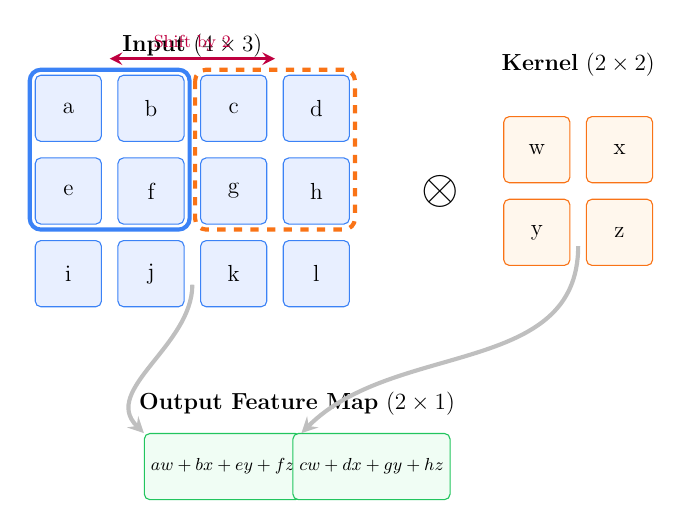
\begin{tikzpicture}[scale=0.7, every node/.style={transform shape}]
    % Color Palette
    \definecolor{inputColor}{HTML}{E8EFFF}
    \definecolor{inputBorder}{HTML}{3B82F6}
    \definecolor{kernelColor}{HTML}{FFF7ED}
    \definecolor{kernelBorder}{HTML}{F97316}
    \definecolor{outputColor}{HTML}{F0FDF4}
    \definecolor{outputBorder}{HTML}{22C55E}
    
    % --- Input Matrix (Top Left) ---
    \begin{scope}[shift={(0,0)}]
        \node[above] at (2.25, 0.8) {\large \textbf{Input} ($4 \times 3$)};
        
        \node[draw=inputBorder, fill=inputColor, minimum size=1.2cm, rounded corners=2pt, font=\large] (a) at (0,0) {a};
        \node[draw=inputBorder, fill=inputColor, minimum size=1.2cm, rounded corners=2pt, font=\large] (b) at (1.5,0) {b};
        \node[draw=inputBorder, fill=inputColor, minimum size=1.2cm, rounded corners=2pt, font=\large] (c) at (3,0) {c};
        \node[draw=inputBorder, fill=inputColor, minimum size=1.2cm, rounded corners=2pt, font=\large] (d) at (4.5,0) {d};
        
        \node[draw=inputBorder, fill=inputColor, minimum size=1.2cm, rounded corners=2pt, font=\large] (e) at (0,-1.5) {e};
        \node[draw=inputBorder, fill=inputColor, minimum size=1.2cm, rounded corners=2pt, font=\large] (f) at (1.5,-1.5) {f};
        \node[draw=inputBorder, fill=inputColor, minimum size=1.2cm, rounded corners=2pt, font=\large] (g) at (3,-1.5) {g};
        \node[draw=inputBorder, fill=inputColor, minimum size=1.2cm, rounded corners=2pt, font=\large] (h) at (4.5,-1.5) {h};
        
        \node[draw=inputBorder, fill=inputColor, minimum size=1.2cm, rounded corners=2pt, font=\large] (i) at (0,-3) {i};
        \node[draw=inputBorder, fill=inputColor, minimum size=1.2cm, rounded corners=2pt, font=\large] (j) at (1.5,-3) {j};
        \node[draw=inputBorder, fill=inputColor, minimum size=1.2cm, rounded corners=2pt, font=\large] (k) at (3,-3) {k};
        \node[draw=inputBorder, fill=inputColor, minimum size=1.2cm, rounded corners=2pt, font=\large] (l) at (4.5,-3) {l};
    \end{scope}

    % Highlight first position
    \draw[inputBorder, line width=1.5pt, rounded corners=4pt] (-0.7,0.7) rectangle (2.2,-2.2);

    % Highlight second position (Stride 2 shift)
    \draw[kernelBorder, dashed, line width=1.5pt, rounded corners=4pt] (2.3,0.7) rectangle (5.2,-2.2);

    % Visual stride jump note
    \draw[<->, >=stealth, line width=1pt, purple] (0.75, 0.9) -- (3.75, 0.9) node[midway, above, font=\small] {Shift by 2};

    % --- Kernel (Top Right) ---
    \begin{scope}[shift={(8.5, -0.75)}]
        \node[above] at (0.75, 1.2) {\large \textbf{Kernel} ($2 \times 2$)};
        \node[draw=kernelBorder, fill=kernelColor, minimum size=1.2cm, rounded corners=2pt, font=\large] (w) at (0,0) {w};
        \node[draw=kernelBorder, fill=kernelColor, minimum size=1.2cm, rounded corners=2pt, font=\large] (x) at (1.5,0) {x};
        \node[draw=kernelBorder, fill=kernelColor, minimum size=1.2cm, rounded corners=2pt, font=\large] (y) at (0,-1.5) {y};
        \node[draw=kernelBorder, fill=kernelColor, minimum size=1.2cm, rounded corners=2pt, font=\large] (z) at (1.5,-1.5) {z};
    \end{scope}

    \node at (6.75, -1.5) {\Huge $\otimes$};

    % --- Output Matrix (Bottom) ---
    \begin{scope}[shift={(2.8, -6.5)}]
        \node[above] at (1.35, 0.8) {\large \textbf{Output Feature Map} ($2 \times 1$)};
        
        \node[draw=outputBorder, fill=outputColor, minimum width=2.5cm, minimum height=1.2cm, rounded corners=2pt, font=\small] (o1) at (0,0) {$aw+bx+ey+fz$};
        \node[draw=outputBorder, fill=outputColor, minimum width=2.5cm, minimum height=1.2cm, rounded corners=2pt, font=\small] (o2) at (2.7,0) {$cw+dx+gy+hz$};
    \end{scope}

    % Arrows
    \draw[->, >=stealth, line width=1.5pt, gray!50] (2.25, -3.2) to[out=-90, in=135] (o1.north west);
    \draw[->, >=stealth, line width=1.5pt, gray!50] (9.25, -2.5) to[out=-90, in=45] (o1.north east);

\end{tikzpicture}
\end{center}

\end{frame}


%% Slide: Transposed Convolution Visualization
\begin{frame}
\frametitle{Transposed Convolution (Upsampling)}

\begin{columns}[T]
\begin{column}{0.4\textwidth}
\textbf{The Mechanism:}
\begin{itemize}
    \item \textbf{Broadcast:} Each input pixel multiplies the entire kernel.
    \item \textbf{Stride:} Determines the spacing between patches.
    \item \textbf{Effect:}
    \begin{itemize}
        \only<1>{\item \textbf{Stride 2:} Increases resolution by spacing patches apart (No overlap with 2x2 kernel).}
        \only<2->{\item \textbf{Stride 1:} Overlaps patches; overlapping regions are \textbf{summed}.}
    \end{itemize}
\end{itemize}

\vspace{0.5cm}
\centering
\begin{tikzpicture}[scale=0.7]
    \only<1>{\draw[thick, ->, blue] (0,0) -- (1,0) node[right, font=\tiny] {Stride 2: High Expansion};}
    \only<2->{\draw[thick, ->, red] (0,0) -- (1,0) node[right, font=\tiny] {Stride 1: Dense Overlap};}
\end{tikzpicture}
\end{column}

\begin{column}{0.6\textwidth}
\centering
\begin{tikzpicture}[scale=0.6]
    % Styles
    \tikzset{
        inp/.style={rectangle, draw, minimum size=0.8cm, font=\small\bfseries},
        ker/.style={rectangle, draw, minimum size=0.6cm, fill=gray!20, font=\tiny},
        outc/.style={rectangle, draw, minimum size=0.75cm, font=\tiny, align=center},
        arr/.style={->, >=stealth, thick, gray!40}
    }

    % 1. Input (Top)
    \node[inp, fill=blue!30] (ia) at (0,7.5) {a};
    \node[inp, fill=red!30] (ib) at (1,7.5) {b};
    \node[inp, fill=yellow!30] (ic) at (0,6.5) {c};
    \node[inp, fill=green!30] (id) at (1,6.5) {d};
    \node[above=0.1cm] at (0.5,7.9) {\footnotesize Input ($2\times2$)};

    % 2. Kernel (Top Right)
    \node[ker] (kw) at (4,7.5) {w};
    \node[ker] (kx) at (4.7,7.5) {x};
    \node[ker] (ky) at (4,6.8) {y};
    \node[ker] (kz) at (4.7,6.8) {z};
    \node[above=0.1cm] at (4.35,7.9) {\footnotesize Kernel ($2\times2$)};

    % Directional Arrows
    \draw[arr] (1.5, 7.0) -- (3, 7.0) node[midway, above, font=\tiny, black] {Broadcast};

    % 3. Output Grid Toggle
    \begin{scope}[shift={(0.2, -0.5)}]
        \only<1>{
            \node[anchor=south] at (2, 4.5) {\footnotesize Output ($4\times4$) via Stride 2};
            \draw[step=1cm, gray!15] (0,0) grid (4,4);
            
            % Stride 2 patches
            \node[outc, fill=blue!10] at (0.5, 3.5) {aw}; \node[outc, fill=blue!10] at (1.5, 3.5) {ax};
            \node[outc, fill=blue!10] at (0.5, 2.5) {ay}; \node[outc, fill=blue!10] at (1.5, 2.5) {az};
            
            \node[outc, fill=red!10] at (2.5, 3.5) {bw}; \node[outc, fill=red!10] at (3.5, 3.5) {bx};
            \node[outc, fill=red!10] at (2.5, 2.5) {by}; \node[outc, fill=red!10] at (3.5, 2.5) {bz};
            
            \node[outc, fill=yellow!10] at (0.5, 1.5) {cw}; \node[outc, fill=yellow!10] at (1.5, 1.5) {cx};
            \node[outc, fill=yellow!10] at (0.5, 0.5) {cy}; \node[outc, fill=yellow!10] at (1.5, 0.5) {cz};

            \node[outc, fill=green!10] at (2.5, 1.5) {dw}; \node[outc, fill=green!10] at (3.5, 1.5) {dx};
            \node[outc, fill=green!10] at (2.5, 0.5) {dy}; \node[outc, fill=green!10] at (3.5, 0.5) {dz};
            
            \draw[<->, purple, thick] (1.5, 4.1) -- (2.5, 4.1) node[midway, above, font=\tiny] {Stride=2};
        }
        \only<2->{
            \node[anchor=south] at (1.5, 4.5) {\footnotesize Output ($3\times3$) via Stride 1};
            \draw[step=1cm, gray!15] (0,0) grid (3,3);
            
            % Stride 1 patches with overlap
            \node[outc, fill=blue!10] at (0.5, 2.5) {aw};
            \node[outc, fill=purple!20] at (1.5, 2.5) {ax+\\bw};
            \node[outc, fill=red!10] at (2.5, 2.5) {bx};
            
            \node[outc, fill=cyan!20] at (0.5, 1.5) {ay+\\cw};
            \node[outc, fill=gray!40] at (1.5, 1.5) {az+by\\+cx+dw};
            \node[outc, fill=orange!20] at (2.5, 1.5) {bz+\\dx};
            
            \node[outc, fill=yellow!10] at (0.5, 0.5) {cy};
            \node[outc, fill=pink!20] at (1.5, 0.5) {cz+\\dy};
            \node[outc, fill=green!10] at (2.5, 0.5) {dz};
            
            \draw[<->, purple, thick] (0.5, 3.5) -- (1.5, 3.5) node[midway, above, font=\tiny] {Stride=1};
        }
    \end{scope}


    \end{tikzpicture}
\end{column}
\end{columns}

\begin{flushleft}
\tiny
\textbf{Summary:}\\
Stride $\geq$ Kernel: Sparse\\
Stride $<$ Kernel: Overlap
\end{flushleft}

\only<3->{
\vspace{-0.5cm}
\begin{flushleft}
\tiny
\textcolor{red}{\textbf{Question:} What happens if Stride = 0? What if Stride = 3?}
\end{flushleft}
}

\end{frame}





\subsection{Historical Milestones (1990s-2026)}
%%% 1990s: LeNet Evolution %%%
\begin{frame}
\frametitle{1990s: LeNet's CNN Breakthrough}

\begin{columns}[T]
\begin{column}{0.6\textwidth}
\textbf{Architectural Innovations:}
\begin{itemize}
\item \textbf{1989:} LeNet-1 (AT\&T Bell Labs)
\begin{itemize}
\item 3 hidden layers, 9,760 parameters
\item 1\% error on USPS zip codes
\end{itemize}

\item \textbf{1998:} LeNet-5
\begin{itemize}
\item 2 Conv + 2 Pool + 3 FC layers
\item MNIST benchmark: 0.8\% error
\item First practical deployment in check reading systems
\end{itemize}
\end{itemize}

\begin{table}
\centering
\scalebox{0.7}{
\begin{tabular}{|l|c|c|c|}
\hline
\textbf{Version} & \textbf{Params} & \textbf{Error} & \textbf{Dataset} \\
\hline
LeNet-1 (1989) & 9,760 & 1\% & USPS \\
LeNet-4 (1994) & 17,000 & 0.7\% & MNIST \\
LeNet-5 (1998) & 60,000 & 0.8\% & MNIST \\
\hline
\end{tabular}
}
\end{table}
\end{column}

\begin{column}{0.4\textwidth}
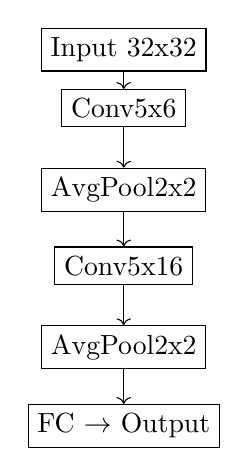
\begin{tikzpicture}[scale=0.5]
\node[draw] (input) {Input 32x32};
\node[draw,below=0.5cm] (conv1) at (0,0) {Conv5x6};
\node[draw,below=0.5cm] (pool1) at (0,-2) {AvgPool2x2};
\node[draw,below=0.5cm] (conv2) at (0,-4) {Conv5x16};
\node[draw,below=0.5cm] (pool2) at (0,-6) {AvgPool2x2};
\node[draw,below=0.5cm] (fc) at (0, -8) {FC $\rightarrow$ Output};

\draw[->] (input) -- (conv1);
\draw[->] (conv1) -- (pool1);
\draw[->] (pool1) -- (conv2);
\draw[->] (conv2) -- (pool2);
\draw[->] (pool2) -- (fc);
\end{tikzpicture}
\end{column}
\end{columns}
\end{frame}


%%% 2012: AlexNet Revolution %%%
\begin{frame}
\frametitle{2012: AlexNet's ImageNet Domination}

\begin{columns}[T]
\begin{column}{0.5\textwidth}
\textbf{ILSVRC 2012 Results:}
\begin{itemize}
\item Top-5 error: 15.3\% (vs 26.2\% second place)
\item 60M parameters, 5 Conv + 3 FC layers
\end{itemize}

\textbf{Key Innovations:}
\begin{itemize}
\item ReLU activation: \( f(x) = \max(0,x) \)
\item Dropout regularization (p=0.5)
\item Dual GPU implementation
\end{itemize}

\begin{table}
\centering
\scalebox{0.7}{
\begin{tabular}{|l|c|}
\hline
\textbf{Model} & \textbf{Top-5 Error} \\
\hline
AlexNet & 15.3\% \\
SVM & 26.2\% \\
Best 2011 Entry & 25.8\% \\
\hline
\end{tabular}
}
\end{table}
\end{column}

\begin{column}{0.5\textwidth}
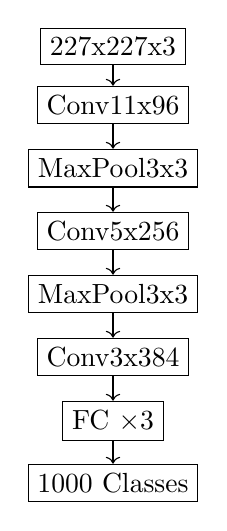
\begin{tikzpicture}[scale=0.4]
\node[draw] (input) {227x227x3};
\node[draw,below=0.5cm] (conv1) at (0,0) {Conv11x96};
\node[draw,below=0.5cm] (pool1) at (0,-2) {MaxPool3x3};
\node[draw,below=0.5cm] (conv2) at (0,-4) {Conv5x256};
\node[draw,below=0.5cm] (pool2) at (0,-6) {MaxPool3x3};
\node[draw,below=0.5cm] (conv3) at (0,-8) {Conv3x384};
\node[draw,below=0.5cm] (fc) at (0,-10) {FC $\times$3};
\node[draw,below=0.5cm] (out) at (0, -12) {1000 Classes};

\draw[->] (input) -- (conv1);
\draw[->] (conv1) -- (pool1);
\draw[->] (pool1) -- (conv2);
\draw[->] (conv2) -- (pool2);
\draw[->] (pool2) -- (conv3);
\draw[->] (conv3) -- (fc);
\draw[->] (fc) -- (out);
\end{tikzpicture}
\end{column}
\end{columns}
\end{frame}



%% Slide 8: Key Milestones in Deep Learning
\begin{frame}
\frametitle{Key Milestones in Deep Learning}
\begin{itemize}
    \item \textbf{2012:} AlexNet demonstrates power of deep CNNs \textit{(~60-62 million parameters)}
    \item \textbf{2014:} GANs introduced by Goodfellow et al.
    \item \textbf{2014:} Encoder-decoder architectures for sequence tasks \textit{(seq2seq: 384M parameters)}
    \item \textbf{2015-16:} ResNet and batch normalization \textit{(ResNet-50: ~25 million parameters)}
    \item \textbf{2017:} Transformer architecture
    \item \textbf{2018-20:} Pre-trained language models
        \begin{itemize}
            \item BERT-Base: 108.8 million parameters
            \item GPT-3: 175 billion parameters
        \end{itemize}
    \item \textbf{2021-present:} Large-scale generative models
        \begin{itemize}
            \item DALL-E: 12 billion parameters
            \item DALL-E 2: 3.5 billion parameters
            \item Stable Diffusion 3.5 Large: 8.1 billion parameters
            \item GPT-4: estimated 1.8 trillion parameters
        \end{itemize}
\end{itemize}
\end{frame}


%%% 2014-Present: Deep Learning Explosion %%%
\begin{frame}
\frametitle{2014-Present: Generative AI Revolution}

\begin{columns}[T]
\begin{column}{0.5\textwidth}
\textbf{Key Developments:}
\begin{itemize}
\item \textbf{2013:} VAEs (Variational Auto-encoding)
\item \textbf{2014:} GANs (Generative Adversarial Networks)
\item \textbf{2015:} ResNets (152 layers)
\item \textbf{2017:} Transformer Architecture (Auto-regressive Gen AI)
\item \textbf{2020:} Diffusion Models, VQ-VAE
\item \textbf{2022:} ChatGPT (175B params), RVQ
\item \textbf{2024:-} Multimodal LLMs, Agentic LLMs
\end{itemize}
\end{column}


\begin{column}{0.5\textwidth}
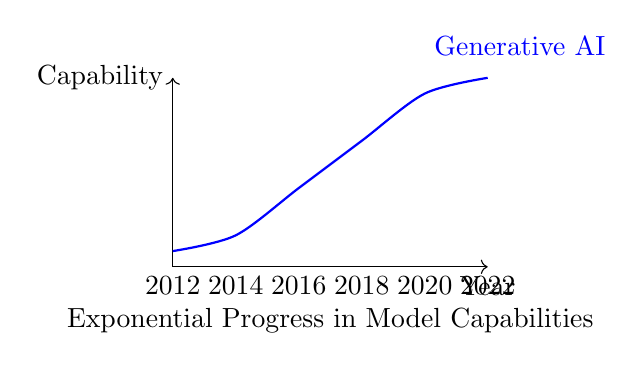
\begin{tikzpicture}[scale=0.4]
\draw[->] (0,0) -- (10,0) node[below] {Year};
\draw[->] (0,0) -- (0,6) node[left] {Capability};

\foreach \x/\y in {2012/1, 2014/2, 2016/3, 2018/4, 2020/5, 2022/6} {
    \node[below] at (\x-2012,0) {\x};
}

\draw[blue,thick] plot[smooth] coordinates {
    (0,0.5)(2,1)(4,2.5)(6,4)(8,5.5)(10,6)
};

\node[blue,right] at (8,7) {Generative\ AI};
\node[below] at (5,-1) {Exponential Progress in Model Capabilities};
\end{tikzpicture}
\textbf{Performance Growth:}
\begin{itemize}
\item Compute: 10x/year since 2012
\item Model size: 5700x increase (2012-2023)
\end{itemize}
\end{column}
\end{columns}


\end{frame}






\section{Mathematical Foundations}
\subsection{Probability Basics}
%%% Slide 1: Probability Basics %%%
\begin{frame}{Core Probability Concepts}
\begin{columns}[T]
\begin{column}{0.48\textwidth}
\textbf{Key Definitions:}
\begin{itemize}
\item \textbf{Sample Space} ($\Omega$): All possible outcomes
\item \textbf{Event} ($E \subseteq \Omega$): Subset of outcomes
\item \textbf{Probability}: $P(E) \in [0,1]$ with:
\begin{itemize}
\item $P(\Omega) = 1$
\item $P(\bigcup_i E_i) = \sum_i P(E_i)$ for disjoint events
\end{itemize}
\end{itemize}
\end{column}

\begin{column}{0.48\textwidth}
\textbf{Random Variables:}
\begin{itemize}
\item Maps outcomes to numbers
\item Discrete vs Continuous
\item PMF/PDF: $p_X(x) = P(X=x)$
\end{itemize}

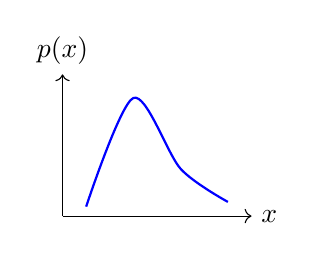
\begin{tikzpicture}[scale=0.6]
\draw[->] (0,0) -- (4,0) node[right] {$x$};
\draw[->] (0,0) -- (0,3) node[above] {$p(x)$};
\draw[blue,thick] plot[smooth] coordinates {(0.5,0.2) (1.5,2.5) (2.5,1) (3.5,0.3)};
\end{tikzpicture}
\end{column}
\end{columns}

\vspace{0.5cm}
\textbf{GenAI Connection:} All generative models learn probability distributions $p(x)$ over data space
\end{frame}

%%% Slide 2: Key Distributions %%%
\begin{frame}{Essential Probability Distributions}
\begin{columns}[T]
\begin{column}{0.33\textwidth}
\textbf{Bernoulli:}
\[ P(X=k) = \begin{cases}
p & k=1 \\
1-p & k=0
\end{cases} \]
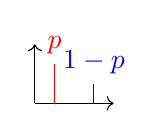
\begin{tikzpicture}[scale=0.5]
\draw[->] (0,0) -- (2,0);
\draw[->] (0,0) -- (0,1.5);
\draw[red] (0.5,0) -- (0.5,1) node[above] {$p$};
\draw[blue] (1.5,0) -- (1.5,0.5) node[above] {$1-p$};
\end{tikzpicture}
\end{column}

\begin{column}{0.33\textwidth}
\textbf{Categorical:}
\[ P(X=k) = p_k \]
\[ \text{where } \sum p_k = 1 \]
\begin{tikzpicture}[scale=0.5]
\foreach \x/\h in {0.5/1.5,1.5/1,2.5/0.8} {
    \draw[blue] (\x,0) -- (\x,\h);
}
\end{tikzpicture}
\end{column}

\begin{column}{0.33\textwidth}
\textbf{Gaussian:}
\[ p(x) = \frac{1}{\sigma\sqrt{2\pi}}e^{-\frac{(x-\mu)^2}{2\sigma^2}} \]
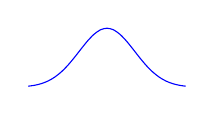
\begin{tikzpicture}[scale=0.5]
\draw[domain=-2:2,smooth,variable=\x,blue] plot ({\x+1.5},{1.5*exp(-\x*\x)});
\end{tikzpicture}
\end{column}
\end{columns}

\vspace{0.5cm}
\textbf{GenAI Usage:} Bernoulli/Categorical for discrete data, Gaussian for continuous latent spaces
\end{frame}

%%% Slide 3: Conditional Probability & Bayes %%%
\begin{frame}{Conditional Probability \& Bayes' Rule}
\textbf{Intuition:} How we update our beliefs when we see new evidence.
\begin{columns}[T]
\begin{column}{0.6\textwidth}
\textbf{Conditional Probability:}
\[ P(A|B) = \frac{P(A \cap B)}{P(B)} \]

\textbf{Bayes' Theorem:}
\[ P(A|B) = \frac{P(B|A)P(A)}{P(B)} \]

\textbf{Chain Rule:}
\[ P(X_1,\ldots,X_n) = \prod_{i=1}^n P(X_i|X_1,\ldots,X_{i-1}) \]
\end{column}

\begin{column}{0.4\textwidth}
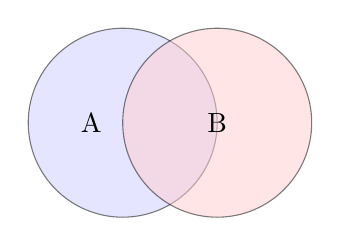
\begin{tikzpicture}[scale=0.8]
\draw[fill=blue!20, opacity=0.5] (0,0) circle (1.5);
\draw[fill=red!20, opacity=0.5] (1.5,0) circle (1.5);
\node at (-0.5,0) {A};
\node at (1.5,0) {B};
\end{tikzpicture}
\vspace{0.5cm}
\newline
\textbf{GenAI Application:} Foundation of latent variable models like VAEs:
\[ p(x|z) = \frac{p(z|x)p(x)}{p(z)} \]
\end{column}
\end{columns}


\end{frame}

\subsection{Parameter Estimation}
%%% Slide 4: Maximum Likelihood Estimation %%%
\begin{frame}{Maximum Likelihood Estimation (MLE)}
\textbf{Intuition:} Finding the parameters that make the observed data most likely.
\begin{columns}[T]
\begin{column}{0.6\textwidth}
\textbf{Objective:}
\[ \theta^* = \arg\max_\theta \prod_{i=1}^N p(x_i|\theta) \]

\textbf{Log-Likelihood:}
\[ \mathcal{L}(\theta) = \sum_{i=1}^N \log p(x_i|\theta) \]

\textbf{Example (Coin Toss):}
\[ \hat{p} = \frac{\text{\# Heads}}{N} \]
\end{column}

\begin{column}{0.4\textwidth}
\begin{tikzpicture}[scale=0.7]
\draw[->] (-1.5,0) -- (1.5,0);
\foreach \x in {-1,0,1} {
    \draw (\x,0) -- (\x,-0.1) node[below] {$\x$};
}
\draw[blue,thick] (0.6,0) -- (0.6,1.5);
\node[blue] at (0.6,1.8) {$\hat{p}$};
\end{tikzpicture}

\vspace{0.5cm}
\textbf{GenAI Connection:} Foundation for training most generative models:
\begin{itemize}
\item Explicit models: Directly maximize likelihood
\item Implicit models: Adversarial training objectives
\end{itemize}
\end{column}
\end{columns}
\end{frame}

%%% Slide 8: From Probability to GenAI %%%
\begin{frame}{Connecting Probability to Generative AI}
\begin{center}
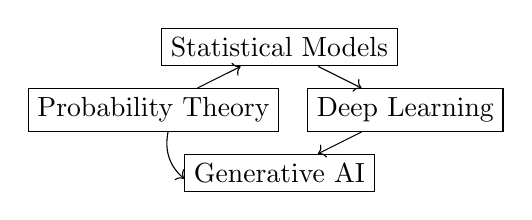
\begin{tikzpicture}[scale=0.8]
\node[draw] (prob) at (0,0) {Probability Theory};
\node[draw] (stats) at (2,1) {Statistical Models};
\node[draw] (dl) at (4,0) {Deep Learning};
\node[draw] (genai) at (2,-1) {Generative AI};

\draw[->] (prob) -- (stats);
\draw[->] (stats) -- (dl);
\draw[->] (dl) -- (genai);
\draw[->] (prob) edge[bend right] (genai);
\end{tikzpicture}
\end{center}

\textbf{Key Connections:}
\begin{itemize}
\item Neural networks $\rightarrow$ flexible function approximators
\item Gradient-based optimization of probabilistic objectives
\item Scalable inference $\rightarrow$ stochastic sampling methods
\end{itemize}
\end{frame}

\section{Introduction to Generative AI}
\subsection{Generative vs Discriminative}
%% Slide 18: Introduction to Generative AI
\begin{frame}
\frametitle{Introduction to Generative AI}
\begin{itemize}
    \item Models that create new content rather than classify/predict
    \item Can generate images, text, audio, video, 3D models, etc.
    \item Learn underlying data distributions
    \item Represent a fundamental shift from discriminative to creative AI
    \item Applications across art, design, content creation, science, and more
\end{itemize}
\end{frame}

%% Slide 19: Discriminative vs. Generative Models
\begin{frame}
\frametitle{Discriminative vs. Generative Models}
\begin{columns}
\begin{column}{0.48\textwidth}
\textbf{Discriminative Models:}
\begin{itemize}
    \item \textbf{Learn} decision \textbf{boundaries} between classes
    \item<2-> Model $P(Y|X)$ - probability of label given input
    \item<3-> Focus on classification/regression tasks
    \item<4-> Examples: CNN classifiers, logistic regression
\end{itemize}
\end{column}
\begin{column}{0.48\textwidth}
\textbf{Generative Models:}
\begin{itemize}
    \item \textbf{Learn} to generate data resembling training \textbf{distribution}
    \item<2-> Model $P(X)$ or $P(X,Y)$ - probability of data (and labels)
    \item<3-> Can create new instances from learned distribution
    \item<4-> Examples: GANs, VAEs, diffusion models
\end{itemize}
\end{column}
\end{columns}

\end{frame}

%% Slide 20: Examples of Discriminative & Generative Tasks
\begin{frame}
\frametitle{Examples of Discriminative \& Generative Tasks}
\begin{columns}
\begin{column}{0.48\textwidth}
\textbf{Discriminative Examples:}
\begin{itemize}
    \item \textbf{MNIST Classification:} 
    \begin{itemize}
        \item Input: Handwritten digit image
        \item Output: Probability over 10 classes
        \item Model: $P(digit|image)$
    \end{itemize}
    \item \textbf{Speaker Identification:}
    \begin{itemize}
        \item Input: Voice recording
        \item Output: Speaker identity
        \item Model: $P(speaker|audio)$
    \end{itemize}
\end{itemize}
\end{column}

\begin{column}{0.48\textwidth}
\textbf{Generative Examples:}
\begin{itemize}
    \item \textbf{Image Generation:}
    \begin{itemize}
        \item Input: Random noise/text prompt
        \item Output: Novel synthetic image 
        \item Model: $P(image)$ or $P(image|text)$
    \end{itemize}
    \item \textbf{Speech Recognition (ASR):}
    \begin{itemize}
        \item Input: Audio waveform
        \item Output: Text transcript
        \item Model: $P(text|audio)$
    \end{itemize}
\end{itemize}
\end{column}
\end{columns}

\begin{center}
\begin{tabular}{|l|c|c|}
\hline
\textbf{Domain} & \textbf{Discriminative Task} & \textbf{Generative Task} \\
\hline
Image & Object Detection & Image Synthesis \\
Speech & Speaker ID & Speech Generation \\
Text & Sentiment Analysis & Text Generation \\
\hline
\end{tabular}
\end{center}

\textbf{Key Insight:} Many tasks can be approached from either perspective!
\end{frame}

\begin{frame}
\frametitle{Generative Models: From Traditional ML to Deep Learning}

\begin{itemize}
\item \textbf{Evolution of Generative Capability:} Generative models have evolved from simple statistical models to complex neural architectures capable of creating highly realistic content.

\item \textbf{Key Evolutionary Stages:}
  \begin{itemize}
  \item \textbf{Statistical Era (1980s-2000s):} Gaussian Mixture Models, Hidden Markov Models
  \item \textbf{Energy-Based Models (2000s):} Restricted Boltzmann Machines, Deep Belief Networks
  \item \textbf{Modern Deep Generative Era (2014-present):} VAEs, GANs, Diffusion Models, Transformers
  \end{itemize}

\item \textbf{Architectural Patterns:} Most successful generative models share key principles:
  \begin{itemize}
  \item Latent space representations (compression of data distributions)
  \item Hierarchical feature learning (from pixels to concepts)
  \item Iterative refinement (progressive improvement of generations)
  \end{itemize}
\end{itemize}
\end{frame}


\begin{frame}
\frametitle{Generative Models: From Traditional ML to Deep Learning}

\begin{itemize}

\item \textbf{Convergence with Other Fields:} Recent generative AI success comes from:
  \begin{itemize}
  \item Large-scale pre-training (foundation models)
  \item Multimodal integration (text, image, audio)
  \item Human feedback and alignment techniques
  \end{itemize}
\end{itemize}
\end{frame}
%% Slide 20: Probabilistic Modeling Foundations
\begin{frame}
\frametitle{Probabilistic Modeling Foundations}
\begin{itemize}
    \item Generative models based on probability theory
    \item Core concept: modeling data distribution $P(X)$
    \item Two main approaches:
    \begin{itemize}
        \item Explicit density estimation (direct modeling)
        \item Implicit density estimation (sampling-based)
    \end{itemize}
    \item Maximum likelihood principle: find parameters that maximize probability of observed data
\end{itemize}

\begin{center}
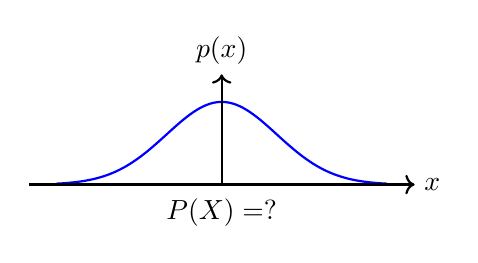
\begin{tikzpicture}[scale=0.7]
    % Draw normal distribution curve
    \draw[domain=-3:3, samples=100, smooth, variable=\x, blue, thick] 
        plot ({\x}, {1.5*exp(-(\x)^2/2)});
    
    % X-axis
    \draw[->, thick] (-3.5,0) -- (3.5,0);
    \node[right] at (3.5,0) {$x$};
    
    % Y-axis
    \draw[->, thick] (0,0) -- (0,2);
    \node[above] at (0,2) {$p(x)$};
    
    % Label
    \node at (0,-0.5) {$P(X) = ?$};
\end{tikzpicture}
\begin{figure}
    \centering
    
\includegraphics[width=0.5\linewidth]{images/image2.png}
    \caption{Empirical Data Distribution vs. Theoretical PDF}
    \label{fig:enter-label}
\end{figure}
\end{center}
\end{frame}

\subsection{Latent Spaces \& Core Concepts}
%% Slide 21: Latent Representations
\begin{frame}
\frametitle{Latent Representations and Spaces}
\begin{itemize}
    \item \textbf{Latent Space:} Lower-dimensional space encoding key features
    \item High-dimensional data $\rightarrow$ compressed representation $\rightarrow$ reconstruction
    \item Properties of good latent spaces:
    \begin{itemize}
        \item Continuous
        \item Complete (covers training distribution)
        \item Disentangled (separable factors of variation)
    \end{itemize}
    \item Enable controlled generation and manipulation
\end{itemize}
\end{frame}





%% Slide 25: Evolution of Generative Capabilities
\begin{frame}
\frametitle{Evolution of Generative Capabilities}
\begin{center}
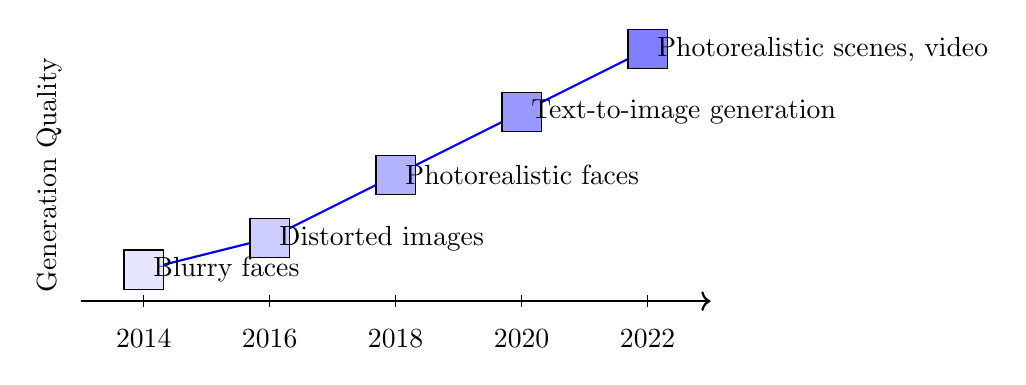
\begin{tikzpicture}[scale=0.8]
    % Draw timeline
    \draw[->, thick] (0,0) -- (10,0);
    
    % Timeline markers
    \foreach \x/\year in {1/2014, 3/2016, 5/2018, 7/2020, 9/2022} {
        \draw (\x,0.1) -- (\x,-0.1);
        \node[below] at (\x,-0.3) {\year};
    }
    
    % Quality improvement
    \draw[blue, thick] (1,0.5) -- (3,1) -- (5,2) -- (7,3) -- (9,4);
    
    % Images
    \node[draw, fill=blue!10, minimum size=0.5cm] at (1,0.5) {};
    \node[draw, fill=blue!20, minimum size=0.5cm] at (3,1) {};
    \node[draw, fill=blue!30, minimum size=0.5cm] at (5,2) {};
    \node[draw, fill=blue!40, minimum size=0.5cm] at (7,3) {};
    \node[draw, fill=blue!50, minimum size=0.5cm] at (9,4) {};
    
    % Labels
    \node[right] at (1,0.5) {Blurry faces};
    \node[right] at (3,1) {Distorted images};
    \node[right] at (5,2) {Photorealistic faces};
    \node[right] at (7,3) {Text-to-image generation};
    \node[right] at (9,4) {Photorealistic scenes, video};
    
    % Y-axis
    \node[rotate=90] at (-0.5,2) {Generation Quality};
\end{tikzpicture}
\end{center}
\end{frame}

\section{Autoencoders: Building the Latent Bridge}
\subsection{AE Architecture}
%% Slide 26: Introduction to Autoencoders
\begin{frame}
\frametitle{Introduction to Autoencoders}
\begin{itemize}
    \item Self-supervised neural networks with two parts:
    \begin{itemize}
        \item \textbf{Encoder:} Compresses input to latent representation
        \item \textbf{Decoder:} Reconstructs input from latent representation
    \end{itemize}
    \item Training objective: Minimize reconstruction error
    \item Bridge between supervised learning and generative modeling
    \item Foundation for more advanced generative architectures
\end{itemize}
\end{frame}

%% Slide 27: Autoencoder Architecture
\begin{frame}
\frametitle{Basic Autoencoder Architecture}
\begin{center}
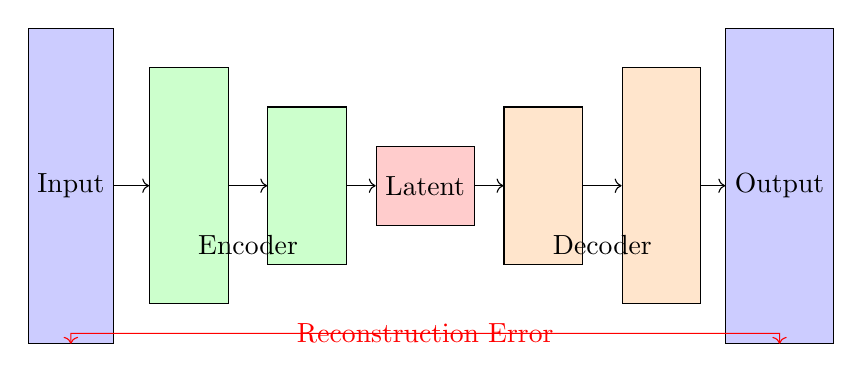
\begin{tikzpicture}[scale=0.75]
    % Input
    \node[rectangle, draw, minimum height=4cm, minimum width=1cm, fill=blue!20] (input) at (0,0) {Input};
    
    % Encoder layers
    \node[rectangle, draw, minimum height=3cm, minimum width=1cm, fill=green!20] (e1) at (2,0) {};
    \node[rectangle, draw, minimum height=2cm, minimum width=1cm, fill=green!20] (e2) at (4,0) {};
    
    % Latent representation
    \node[rectangle, draw, minimum height=1cm, minimum width=1cm, fill=red!20] (latent) at (6,0) {Latent};
    
    % Decoder layers
    \node[rectangle, draw, minimum height=2cm, minimum width=1cm, fill=orange!20] (d1) at (8,0) {};
    \node[rectangle, draw, minimum height=3cm, minimum width=1cm, fill=orange!20] (d2) at (10,0) {};
    
    % Output
    \node[rectangle, draw, minimum height=4cm, minimum width=1cm, fill=blue!20] (output) at (12,0) {Output};
    
    % Connections
    \draw[->] (input) -- (e1);
    \draw[->] (e1) -- (e2);
    \draw[->] (e2) -- (latent);
    \draw[->] (latent) -- (d1);
    \draw[->] (d1) -- (d2);
    \draw[->] (d2) -- (output);
    
    % Labels
    \node[below=0.5cm] at (3,0) {Encoder};
    \node[below=0.5cm] at (9,0) {Decoder};
    
    % Loss
    \draw[<->, red] (input) -- (0,-2.5) -- (12,-2.5) -- (output);
    \node[red] at (6,-2.5) {Reconstruction Error};
\end{tikzpicture}
\end{center}
\end{frame}

%% Slide 28: Types of Autoencoders
\begin{frame}
\frametitle{Types of Autoencoders}
\begin{itemize}
    \item \textbf{Vanilla Autoencoder:} Basic architecture
    \item \textbf{Denoising Autoencoder:} Trained to recover clean data from noisy input
    \item \textbf{Sparse Autoencoder:} Adds sparsity constraint to hidden representations
    \item \textbf{Convolutional Autoencoder:} Uses CNN architectures for images
    \item \textbf{Variational Autoencoder (VAE):} Probabilistic version with regularized latent space
\end{itemize}

\begin{center}
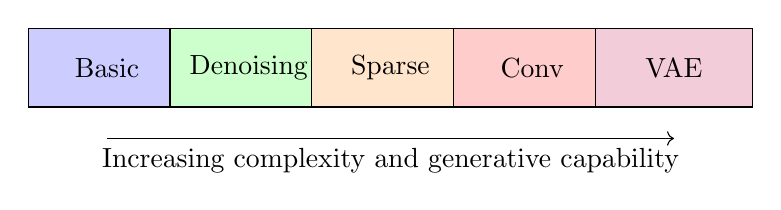
\begin{tikzpicture}[scale=0.6]
    % Autoencoder types diagram
    \node[rectangle, draw, fill=blue!20, minimum width=2cm, minimum height=1cm] (basic) at (0,0) {Basic};
    \node[rectangle, draw, fill=green!20, minimum width=2cm, minimum height=1cm] (denoising) at (3,0) {Denoising};
    \node[rectangle, draw, fill=orange!20, minimum width=2cm, minimum height=1cm] (sparse) at (6,0) {Sparse};
    \node[rectangle, draw, fill=red!20, minimum width=2cm, minimum height=1cm] (conv) at (9,0) {Conv};
    \node[rectangle, draw, fill=purple!20, minimum width=2cm, minimum height=1cm] (vae) at (12,0) {VAE};
    
    % Complexity arrow
    \draw[->] (0,-1.5) -- (12,-1.5);
    \node[below] at (6,-1.5) {Increasing complexity and generative capability};
\end{tikzpicture}
\end{center}
\end{frame}

%% Slide 29: Project Overview
\subsection{Hands-on: Image Reconstruction}
\begin{frame}
\frametitle{Hands-on: Simple Autoencoder for Image Reconstruction}
\begin{itemize}
    \item Click here to download/open the notebook: \attachfile[color=0.5 0.5 0.5]{hands-on/Auto_Encoder_Hands_On.ipynb} (or click \href{run:hands-on/Auto_Encoder_Hands_On.ipynb}{here} to open if supported)
\end{itemize}
\end{frame}


%% Slide 35: Connection to Advanced Generative Models
\begin{frame}
\frametitle{Connection to Advanced Generative Models}
\begin{itemize}
    \item Autoencoders establish \textbf{latent space} concept central to generative AI
    \item VAEs add probabilistic framework for generation
    \item Modern image generators (diffusion models) incorporate similar encoder-decoder structures
    \item Understanding autoencoders provides foundation for:
    \begin{itemize}
        \item GANs
        \item VAEs
        \item Diffusion Models
        \item Transformer-based generative models
    \end{itemize}
\end{itemize}
\end{frame}

\section{Conclusion \& Summary}
%% Slide 36: Session Summary
\begin{frame}
\frametitle{Session Summary}
\begin{itemize}
    \item Explored the evolution from traditional ML to deep learning
    \item Reviewed fundamental neural network architectures
    \item Understood the transition to generative AI paradigm
    \item Implemented a simple autoencoder for image reconstruction
\end{itemize}
\end{frame}



\section{Appendix}
\subsection{Sampling \& Generation}

%%% Slide 7: Sampling Methods %%%
\begin{frame}{Sampling \& Generation}
\begin{columns}[T]
\begin{column}{0.6\textwidth}
\textbf{Key Techniques:}
\begin{itemize}
\item Ancestral Sampling
\item Markov Chain Monte Carlo (MCMC)
\item Importance Sampling
\item Rejection Sampling
\end{itemize}

\textbf{Modern Methods:}
\begin{itemize}
\item Langevin Dynamics
\item Diffusion Process
\item Normalizing Flows
\end{itemize}
\end{column}

\begin{column}{0.4\textwidth}
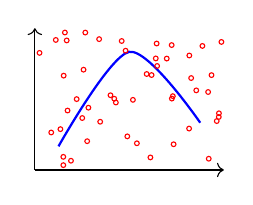
\begin{tikzpicture}[scale=0.6]
\draw[->] (0,0) -- (4,0);
\draw[->] (0,0) -- (0,3);
\draw[blue,thick] plot[smooth] coordinates {(0.5,0.5) (2,2.5) (3.5,1)};
\foreach \i in {1,...,50} {
    \draw[red] (rnd*4, rnd*3) circle (0.05);
}
\end{tikzpicture}
\end{column}
\end{columns}

\vspace{0.5cm}
\textbf{GenAI Application:} All generative models ultimately require efficient sampling from learned distributions
\end{frame}

\end{document}